\label{chap:pt1_chapter6}

Having solved the simplified version of the problem, where fixture rotations  and areas to be extruded are not considered, using the CP model described in Chapter~\ref{chap:pt1_chapter5}, we now address the complete problem by incorporating both fixture rotations  and the presence of areas to be extruded within the workpiece.

The constraints remain the same as those described previously, with the additional requirement that fixtures must not be positioned beneath areas to be extruded. Therefore, the resulting constraints that need to be satisfied are:
\begin{enumerate}
	\item the number of placed fixtures must not exceed their availability;
	\item fixtures must satisfy the minimum safety distances;
	\item fixtures must lie within the boundaries of the workpiece and beneath its surface;
	\item fixtures must not overlap;
	\item fixtures must not be located beneath areas to be extruded.
\end{enumerate}

To clarify layout feasibility, Figure~\ref{fig:constraints_axample} illustrates examples of valid and invalid fixture placements. In the figure, fixture $F_6$ is invalid because it violates the minimum horizontal safety distance with respect to fixtures $F_3$ and $F_4$. Fixture $F_5$, on the other hand, is invalid because it is positioned beneath an area to be extruded.

\begin{figure}[t]
	\centering
	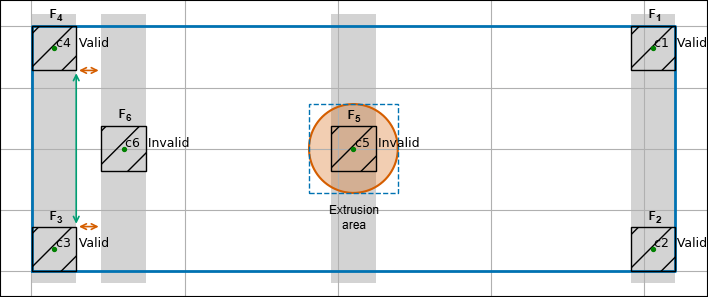
\includegraphics[width=0.65\linewidth]{figures/valid_invalid_positions_example.png}
	\caption{Example of valid and invalid fixture placements. For a fixture placement to be valid, the fixture must lie within the workpiece boundaries, satisfy the required safety distances from the other fixtures, and not be positioned beneath an area to be extruded.}
	\label{fig:constraints_axample}
\end{figure}

To address the complete problem, we extend the CP model introduced in Section~\ref{sec:first_cp_model} to handle the new constraint. We also formulate a new Mixed Integer Programming (MIP) model and propose a Q-learning based algorithm, comparing the three approaches on real-world test cases.

Both the CP and MIP models can be solved using appropriate solvers to obtain feasible layout. However, similarly to the Q-learning algorithm, neither approach accounts for fixture rotations, since allowing rotation angles other than multiples of $90^\circ$ significantly increases the number of possible configurations and makes the problem substantially harder to solve.

Moreover, inclined fixtures complicate overlap checking and, in CP solvers, require geometric approximations due to the lack of native support for continuous variables. For these reasons, fixture rotations are handled in a final refinement stage based on a Particle Swarm Optimization (PSO) meta-heuristic, which iteratively improves the initial solution, provided by the different approaches.

\section{Parameters and objective function}
\label{sec:second_parameters}
The problem parameters extend those introduced in Section~\ref{sec:first_parameters} with information related to the areas to be extruded. 

All the proposed solution strategies are defined over the same set of input parameters, listed below:

\begin{itemize}
	\item the width $\wtab$ and height $\htab$ of the machine worktable;
	\item the minimum horizontal distance $\wmin$ between two fixtures placed on different bars;
	\item the minimum vertical distance $\hmin$ between two fixtures placed on the same bar;
	\item the number $\ntypes$ of different fixture types;
	\item the number $\nfix_i$ of available fixtures for each type $i \in [1..\ntypes]$;
	\item the total number of available fixtures $\nfix = \sum_{i=1}^{\ntypes} \nfix_i$;
	\item the minimum $\nmin$ and maximum $\nmax$ number of fixtures to place;
	\item the width $\wfix_i$ and height $\hfix_i$ of each fixture of type $i$;
	\item the workpiece shape, by a set of linear inequalities of the form $\mathtt{a}\,x + \mathtt{b}\,y + \mathtt{c} \leq 0$;
	\item the number $\numext$ of areas to be extruded;
	\item the width $\ewside_i$, height $\ehside_i$, and the coordinates $(\xext_i, \yext_i)$ of the lower-left corner of the smallest axis-aligned rectangle enclosing each area $i \in [1..\numext]$ to be extruded.
\end{itemize}

To facilitate the solving process, areas to be extruded are approximated by their minimum bounding rectangles. In practice, these areas typically correspond to simple geometries, such as circles, rectangles, or ellipses, while more complex shapes are usually refined manually.

Compared with the simplified formulation, we also introduce in the parameters the minimum vertical distance between fixtures. This parameter was previously omitted to allow the placement of multiple fixtures beneath the workpiece and to facilitate the comparison between $\fdistsemi$ and $\finer$ for increasing values of $\nmax$ (see Section~\ref{sec:case_study}).

To evaluate the quality of a fixture layout, two objective functions are considered $\fdistarea$ and $\finer$. 

The CP and MIP models optimize the objective function $\fdistarea$, which maximizes the sum of the pairwise Manhattan distances between fixture centroids, augmented by the total area of the selected fixtures:

\begin{equation}
	\fdistarea = \sum_{1 \le i < j \le n} \left(|cx_i - cx_j| + |cy_i - cy_j|\right) + \sum_{k=1}^{n} (\wfix_{t_k} \cdot \hfix_{t_k})
	\label{eq:f_dist_area}
\end{equation}

We adopt the area term instead of the semi-perimeter to prioritize fixtures with larger contact surfaces. We empirically verified that this approach provides a stronger surrogate for the inertia objective in more complex geometries. In the experiments of Section~\ref{sec:evaluation}, the Pearson correlation  coefficient~\cite{benesty2009pearson} between $\fdistarea$ and $\finer$ when using the area-based formulation is higher (0.79) than the semi-perimeter-based one (0.39).

Unlike the CP and MIP models, the Q-learning algorithm is not affected by the nonlinear operations required to evaluate $\finer$. Consequently, it does not rely on the alternative objective function; instead, it directly incorporates the moments of inertia into the reward returned by the environment.

\section{CP model}
\label{sec:cp_model}

We formulate the model by extending the CP formulation presented in Section~\ref{sec:first_cp_model} through a revised definition of the decision variables and a reformulation of some constraints, which will be presented in the following sections. 

\subsection{Variables}
\label{sec:second_cp_variables}

The fixture placement and type are represented by three arrays of integer decision variables, $x$, $y$, and $t$, for $i = 1,\ldots,\nmax$:
\begin{itemize}
	\item $ (x_i,y_i) \in [0..\wtab]\times [0..\htab] $ denotes the coordinates of the lower-left corner of the $i$-th fixture;
	\item $ t_i \in [0..\ntypes] $ denotes the type of the $i$-th fixture, where type $0$ represents an unused fixture.
\end{itemize}

For each fixture type $i \in [1..\ntypes]$, an integer variable $n_i \in [0..\nfix_i]$ denotes the number of selected fixtures of type $i$, and a variable $n \in [\nmin..\nmax]$ represents the total number of selected fixtures.

Compared with the formulation presented in~\ref{sec:first_cp_model}, the arrays $x$ and $y$ and the variable $n$ are now bounded by $\nmax$, rather than by $\nfix$, since the maximum number of fixtures that can be placed is known for each workpiece and $\nmax \leq \nfix$ this tighter bound reduces the search space.


\subsection{Constraints}
\label{sec:second_cp_cons}

For each fixture type $i \in [1..\ntypes]$, the \texttt{count} global constraint is used to compute the number of occurrences of value $i$ in the array $t$:

\[
n_i = \texttt{count}(t,i)
\]

The total number of selected fixtures is then defined as

\[
n = \sum_{i=1}^{\ntypes} n_i
\]

Fixture availability is enforced by requiring that the number of selected fixtures of each type does not exceed the number available:

\[
n_i \leq \nfix_i, \qquad \forall i \in [1..\ntypes]
\]

Since not all available fixtures must necessarily be used, we enforce the following invariant:
\[
(i > n) \iff (x_i = \wtab \;\wedge\; y_i = \htab \;\wedge\; t_i = 0), \qquad \forall i \in [1..\nmax]
\]

This invariant ensures that all unused fixtures are assigned the dummy type $0$ and placed at the dummy location $(\wtab,\htab)$, which lies outside the feasible region.

We guarantee that exactly $\nmax-n$ fixtures remain unused by imposing

\[
\texttt{count}(t,0) = \nmax - n
\]


The workpiece shape is defined by linear inequalities of the form $ \mathtt{a}\,x + \mathtt{b}\,y + \mathtt{c} \leq 0 $.
To ensure that each selected fixture $ i $ is placed within the workpiece, we must satisfy
$
\mathtt{a}\,x'_i + \mathtt{b}\,y'_i + \mathtt{c} \leq 0,
$
where $x'_i$ and $y'_i$ are defined as in Section~\ref{sec:first_constraints}.

Areas to be extruded are approximated by axis-aligned rectangles. The non-overlap between these areas and the fixtures is enforced using the \texttt{diffn} global constraint~\cite{DBLP:journals/constraints/BeldiceanuCDP07}:

\[
\texttt{diffn}\big(
x \oplus \xext,\;
y \oplus \yext,\;
[\wfix_{t_i} \mid i \in [1..n]] \oplus \ewside,\;
[\hfix_{t_i} \mid i \in [1..n]] \oplus \ehside
\big)
\]

\noindent where $ \oplus $ denotes array concatenation. Specifically, we use the \emph{non-strict} version of \texttt{diffn}, ignoring the unused fixtures.

To enforce the minimum \emph{vertical} distance $ \hmin $ between fixtures placed on the same bar, and the minimum \emph{horizontal} distance $ \wmin $ between fixtures placed on different bars we impose:

\begin{equation*}
	\begin{aligned}
		&\forall\,1 \le i < j \le n:\quad
		\begin{cases}
			y_i + \hfix_{t_i} + \hmin \le y_j
			\\[-0.2ex]
			\quad\vee\quad
			y_j + \hfix_{t_j} + \hmin \le y_i,
			& \text{if } cx_i = cx_j
			\\[1ex]
			x_i + \wfix_{t_i} + \wmin \le x_j,
			& \text{if } cx_i \ne cx_j
		\end{cases}
	\end{aligned}
\end{equation*}

\noindent where $cx_i$ denotes the $x$-coordinate of the centroid of fixture $ i $. Centroid coordinates are used instead of lower-left coordinates because fixtures may be wider than their supporting bar: while $ x_i $ may fall outside the horizontal span of the bar, the centroid $ cx_i $ always lies within it.

To compute the fixture centroid coordinates while preserving integer-valued variables, the coordinates are obtained using integer division of the fixture dimensions. For each fixture $i \in [1..\nmax]$, we define:

\begin{align*}
	cx_i = x_i + \left\lfloor \frac{\wfix_{t_i}}{2} \right\rfloor \quad
	cy_i = y_i + \left\lfloor \frac{\hfix_{t_i}}{2} \right\rfloor 
\end{align*}

To improve the propagation of the integer division, the following redundant linear constraints were introduced:

\begin{align*}
	2 \cdot cx_i - 2 \cdot x_i = \wfix_{t_i} - (\wfix_{t_i} \bmod 2) \\
	2 \cdot cy_i - 2 \cdot y_i = \hfix_{t_i} - (\hfix_{t_i} \bmod 2)
\end{align*}

Finally, the model exhibits symmetries whenever fixtures of the same type are permuted without changing their spatial arrangement. To eliminate these equivalent solutions, a lexicographic ordering is imposed on the fixture positions using the \texttt{lex\_chain} global constraint:

\[
(x_{i-1},y_{i-1}) \preceq (x_i,y_i)
\qquad i \in [2..\nmax]
\]

\section{MIP model}
\label{sec:mip_model}

In this section, we present the Mixed-Integer Programming (MIP) formulation for the fixture layout optimization problem. Compared to the CP model described in Section~\ref{sec:cp_model}, all the constraints are expressed in linear form, and the positional decision variables are continuous rather than discrete.

This important relaxation comes from the nature of MIP solving which, unlike most CP solvers, naturally handles non-negative continuous variables.
Nevertheless, a number of discrete variables are still required to capture the combinatorial structure of the problem, as detailed below.

\subsection{Variables}
Variables $x_i$ and $y_i$ for $i=1,\dots,\nmax$ have exactly the same semantics as those defined in Section~\ref{sec:second_cp_variables}, with the only difference that they are now continuous reather than discrete.

Fixture types are encoded with a 0-1 matrix $T$ of size $\nmax \times \ntypes$, whose semantics is:
\[
T_{i,j} =
\begin{cases}
	1 & \text{if fixture $i$ is selected and has type $j$,} \\
	0 & \text{otherwise.}
\end{cases}
\]

The linearization of the constraints comes at the expense of the introduction of auxiliary 0-1 variables, detailed as follows:
\begin{itemize}
	\item $\used_i$, denoting whether fixture $i$ is selected;
	\item $\samebar_{i,j}$, denoting whether fixtures $i$ and $j$ lie on the same bar;
	\item $\aboveinbar_{i,j}$, $\belowinbar_{i,j}$, denoting whether fixture $i$ is above or below fixture $j$ on the same bar;
	\item $\nooverlapabove_{i,j}, \nooverlapbelow_{i,j}, \nooverlapleft_{i,j}, \nooverlapright_{i,j}$, indicating whether fixture $i$ is positioned above, below, to the left, or to the right of fixture $j$, respectively.
	\item $\aboveext_{i,j}$, $\belowext_{i,j}$, $\leftext_{i,j}$, $\rightext_{i,j}$ indicating whether fixture $i$ is positioned above, below, to the left, or to the right of an area $j$ to be extruded, respectively.
\end{itemize}

We also define auxiliary variables $w_i$, $h_i$ and $t_i$ to denote, respectively, the width $w_i$, the height $h_i$, and the type $t_i$ of each fixture.

\subsection{Constraints}
For each fixture $i \in [1..\nmax]$ we impose:
\[
\used_i = \sum_{j=1}^{\ntypes} T_{i,j} \qquad
w_i = \sum_{j=1}^{\ntypes} \wfix_j\cdot T_{i,j} \qquad
\]
\[
h_i = \sum_{j=1}^{\ntypes} \hfix_j\cdot T_{i,j} \qquad
t_i = \sum_{j=1}^{\ntypes} j \cdot T_{i,j}
\]

These equations ensure that the width, height, and type assigned to each fixture are consistent and that unused fixtures have dimensions and type equal to $0$.

To enforce availability constraints, we impose:
\[
\sum_{i=1}^{\nmax} T_{i,j} \le \nfix_j, \quad \forall j \in [1..\ntypes] \qquad\qquad
\nmin \le \sum_{i=1}^{\nmax} \used_i \le \nmax
\]

To determine whether two fixtures lie on the same bar for all $i \in [1..\nmax]$ and $j \in [i+1..\nmax]$ we define the following constraints:
\[
\begin{aligned}
	&\samebar_{i,j} \le \used_i \qquad \samebar_{i,j} \le \used_j \\
	&\samebar_{i,j} = \aboveinbar_{i,j} + \belowinbar_{i,j}\\
	&cx_i - cx_j \le M (1 - \samebar_{i,j}) \qquad cx_j - cx_i \le M (1 - \samebar_{i,j}) \\
\end{aligned}
\]

\noindent where $M = \wtab \cdot \htab$ is the \emph{``big-M''} constant. To enforce the appropriate safety distances:

\[
\begin{aligned}
	&cx_i + \wmin \le cx_j + M(\samebar_{i,j} + \nooverlapright_{i,j}) \\
	&cx_j + \wmin \le cx_i + M(\samebar_{i,j} + \nooverlapleft_{i,j}) \\
	&y_i + h_i + \hmin - y_j \le M (1 - \aboveinbar_{i,j}) \\
	&y_j + h_j + \hmin - y_i \le M (1 - \belowinbar_{i,j})
\end{aligned}
\]

To prevent overlap between fixtures, for all $i,j \in [1..\nmax]$ with $i < j$, we impose:
\[
\begin{aligned}
	&\nooverlapabove_{i,j} + \nooverlapbelow_{i,j} +
	\nooverlapleft_{i,j} + \nooverlapright_{i,j} \ge 1 \\
	&x_i + w_i \le x_j + M (1 - \nooverlapleft_{i,j}) \qquad
	&y_i + h_i \le y_j + M (1 - \nooverlapbelow_{i,j}) \\
	&x_j + w_j \le x_i + M (1 - \nooverlapright_{i,j}) \qquad
	&y_j + h_j \le y_i + M (1 - \nooverlapabove_{i,j})
\end{aligned}
\]

The same constraints are applied to prevent overlap between fixtures and areas to be extruded. For each fixture $i \in [1..\nmax]$ and extrusion area $j \in [1..\numext]$, the above inequalities are instantiated using the variables $\aboveext_{i,j}$, $\belowext_{i,j}$, $\leftext_{i,j}$, and $\rightext_{i,j}$.

The workpiece is defined by linear inequalities of the form $\mathtt{a}x_i + \mathtt{b}y_i + \mathtt{c} \leq 0$, so for each fixture $i \in [1..\nmax]$ we impose
$\mathtt{a}x'_i + \mathtt{b}y'_i + \mathtt{c} \leq 0$ where $x'_i$ and $y'_i$ are defined as in Section~\ref{sec:first_constraints}.

To break symmetries, we impose an ordering on fixture types: $t_i \ge t_{i+1}$ for $i \in [1..\nmax-1]$.

\noindent We linearize $\fdistarea$ with a big-M formulation unfolding each term of the form $u=|v|$ into: $$u \ge v ~\wedge~ u \ge -v ~\wedge~ u \leq v + M (1 - b)  ~\wedge~ u \leq -v + M b~\wedge~ b\in\{0,1\}.$$

\section{Q-learning algorithm}

The solutions obtained using the CP and MIP models are compared with those produced by a Q-learning based algorithm. This comparison provides insight into the differences between the layouts generated by exact optimization methods and those obtained through a learning-based strategy.

In Q-learning an agent estimates the action-value function $Q(s,a)$, which represents the expected \emph{cumulative discounted reward} associated with taking action $a$ in state $s$ and subsequently following the optimal policy $\pi$~\cite{watkins1992q}.

In our formulation, the environment corresponds to the considered workpiece. At each decision step, the state of the environment is defined as:

\[
s_t=(n_t,fix_t),
\]

\noindent where $n_t$ is the number of fixtures already placed at step $t$, while
$fix_t=[fix_t^{1},\,fix_t^{2},\\ \,\ldots,\,fix_t^{\ntypes}]$
is an integer array of size $\ntypes$, whose components denote the remaining availability of the different fixture types.

An action consists of selecting a fixture type together with a feasible centroid position:

\[
a_t=(type_t,(cx_t,cy_t)).
\]

The fixture centroid is used as the reference point for positioning instead of the lower-left corner adopted in the CP and MIP models, since it simplifies both the enforcement of the horizontal and vertical safety-distance constraints, as described in Section~\ref{sec:second_cp_cons}, and the identification of feasible actions.

The action to be executed is selected according to an \textit{$\epsilon$-greedy policy}~\cite{sutton1998reinforcement}. At each decision step, the agent selects the action with the highest estimated $Q$-value with probability $1-\epsilon$, whereas with probability $\epsilon$ it selects a random action, balancing exploration and exploitation of the environment.

The Q-learning based procedure adopted for fixture layout optimization is described in Algorithm~\ref{alg:qlearning_fixtures}. The algorithm takes as inputs the number of training episodes $E$, the maximum number of steps per episode $T$, the learning rate $\alpha$, the discount factor $\gamma$, the exploration rate $\epsilon$, and the exploration decay factor $\rho$. The output is the best feasible fixture layout $\mathcal{L}^{*}$ obtained by applying the learned policy $\pi$.

\begin{algorithm}[ht]
	\footnotesize
	\caption{Q-learning for Fixture Layout Optimization}
	\label{alg:qlearning_fixtures}
	\begin{algorithmic}[1]
		
		\Require Number of episodes $E$, maximum number of steps per episode $T$, learning rate $\alpha$, discount factor $\gamma$, exploration rate $\epsilon$, exploration decay factor $\rho$
		\Ensure Best feasible layout $\mathcal{L}^*$
		
		\State Compute all candidate centroid positions
		\label{alg:q_init_start}
		\State Remove centroid positions violating the constraints and set $\mathcal{A}(s_1)$
		\State Initialize $Q(s,a)=0$
		\State $\mathcal{L}^* \gets \emptyset$
		\label{alg:q_init_end}
		
		\For{$ep=1$ to $E$}
		\label{alg:q_iteration_start}
		
		\For{$t=1$ to $T$}
		
		% \State Compute the feasible action set $\mathcal{A}(s_t)$
		
		\If{$\mathcal{A}(s_t)=\emptyset$}
		\State \textbf{break}
		\EndIf
		\label{alg:q_iteration_end}
		
		\If{random number $<\epsilon$} \Comment{exploration}
		\label{alg:q_policy_start}
		\State Select a random feasible action
		$a_t \in \mathcal{A}(s_t)$
		\Else \Comment{exploitation}
		\State Select
		$a_t=\arg\max\limits_{a\in\mathcal{A}(s_t)}Q(s_t,a)$
		\EndIf
		
		\State Perform action $a_t$ by placing the selected fixture
		\label{alg:q_policy_end}
		
		\State Recompute the feasible action set $\mathcal{A}(s_{t+1})$ 
		\label{alg:q_reset_action}
		
		\State Compute reward $r_t$ according to Eq.~\ref{eq:reward}
		\label{alg:q_update_start}
		
		\State Observe successor state $s_{t+1}$
		
		\State $Q(s_t,a_t) \gets Q(s_t,a_t) + \alpha \left[r_{t+1} + \gamma \max_{a_{t+1}}Q(s_{t+1},a_{t+1}) - Q(s_t,a_t) \right]$
		
		\State $s_t \gets s_{t+1}$
		\State Update $\pi$ with $a_t$
		\label{alg:q_update_end}
		
		\EndFor
		
%		\If{$\mathcal{L}_{ep}$ is better than $\mathcal{L}^*$}
%		\label{alg:q_new_ep_start}
%		\State $\mathcal{L}^* \gets \mathcal{L}_{ep}$
%		\EndIf
		\State $\epsilon \gets \rho\,\epsilon$
		\label{alg:q_new_ep_start}
		\State Reset the environment to the initial state $s_1$
		\State Reset the action space to $\mathcal{A}(s_1)$
		\label{alg:q_new_ep_end}
		
		\EndFor
		
		\State Evaluate the learned policy $\pi$
		\label{alg:q_evaluate_start}
		\State \textbf{return} $\mathcal{L}^*$
		\label{alg:q_evaluate_end}
		
	\end{algorithmic}
\end{algorithm}

Given the fixture dimensions, it is known \emph{a priori} that some positions within the workpiece cannot accommodate a fixture, particularly those near the workpiece boundary or close to areas to be extruded. During the initialization phase, in lines~\ref{alg:q_init_start}--\ref{alg:q_init_end} of Algorithm~\ref{alg:qlearning_fixtures}, centroid positions that would result in fixtures extending outside the workpiece boundaries or overlapping areas to be extruded are removed from the set of possible actions $\mathcal{A}(s_t)$, considering the dimensions of the smallest fixture as reference.

\begin{figure}[t]
	\centering
	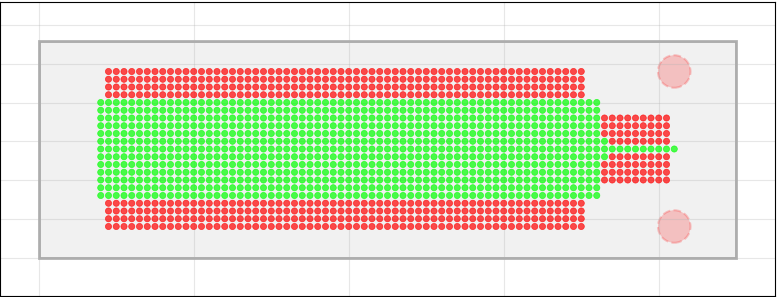
\includegraphics[width=0.5\linewidth]{figures/q_learning_actions.png}
	\caption{Example of the available actions for a given workpiece. Green dots represent centroid positions where both square and rectangular fixtures can be placed, whereas red dots represent positions where only rectangular fixtures can be placed. The workpiece area is highlighted in light gray, while the areas to be extruded are highlighted in red.}
	\label{fig:q_learning_actions}
\end{figure}

Figure~\ref{fig:q_learning_actions} shows an example of the set of feasible actions for a given workpiece, considering two available fixture types: square and rectangular. Green dots indicate centroid positions where both fixture types can be placed, whereas red dots indicate positions where only rectangular fixtures can be placed.

The algorithm iterates over the training episodes and the corresponding steps. An episode terminates when no feasible actions remain or the maximum number of steps is reached, as reported in lines~\ref{alg:q_iteration_start}--\ref{alg:q_iteration_end} of Algorithm~\ref{alg:qlearning_fixtures}.

The agent selects actions according to the $\epsilon$-greedy policy (lines~\ref{alg:q_policy_start}--\ref{alg:q_policy_end} of Algorithm~\ref{alg:qlearning_fixtures}), balancing the exploration of new placements with the exploitation of previously learned actions.

Each action selected is evaluated through the reward associated with the transition from $s_t$ to $s_{t+1}$. The reward function combines the improvement obtained in the moment of inertia with additional terms promoting layouts composed of a larger number of fixtures, larger fixture dimensions, and increased spatial separation between fixtures:

\begin{equation}
	r_{t+1}
	=
	\lambda_{\mathrm{iner}}\,\Delta\finer
	+
	\lambda_n n_{t+1}^{2}
	+
	\lambda_d\bar d
	+
	\begin{cases}
		b_{\nmin}, & \text{if } n_{t+1}\geq\nmin,\\
		0, & \text{otherwise}.
	\end{cases}
	\label{eq:reward}
\end{equation}

\noindent in the equation: 
\begin{itemize} 
	\item $\Delta\finer$ is the variation of $\finer$ between the previous and current states;
	\item $n_{t+1}$ is the number of fixtures in the resulting layout. The quadratic term promotes layouts with a larger number of fixtures;
	\item $\bar d$ is the average Euclidean distance between the newly placed fixture and the previously placed fixtures,  promoting layouts with a larger spatial separation;
	\item $\lambda_{\finer}$, $\lambda_n$, and $\lambda_d$ are weighting coefficients balancing the contribution of the different reward components;
	\item $b_{\nmin}$ is an additional feasibility bonus assigned when the minimum required number of fixtures, $\nmin$, has been placed.
\end{itemize}

After each fixture placement, all candidate centroid positions that no longer satisfy the safety-distance constraints are removed from the feasible action set, as reported in line~\ref{alg:q_reset_action} of Algorithm~\ref{alg:qlearning_fixtures}. Consequently, the action set progressively shrinks as the layout is constructed, ensuring that all geometric constraints are satisfied.

The only constraint that cannot be enforced by restricting the feasible action set is the placement of the minimum number of required fixtures $\nmin$. For this reason, the feasibility bonus $b_{\nmin}$ is included in the reward function to encourage the agent to generate layouts satisfying this constraint.

After executing the selected action, and obtained the corresponding reward, the $Q$-function value associated with state $s_t$ and action $a_t$ is evaluated and the learned policy $\pi$ is updated (lines~\ref{alg:q_update_start}--\ref{alg:q_update_end} of Algorithm~\ref{alg:qlearning_fixtures}).

Once an episode has ended, the environment is arranged for the next episode, as reported in lines~\ref{alg:q_new_ep_start}--\ref{alg:q_new_ep_end} of Algorithm~\ref{alg:qlearning_fixtures}.

Finally, after all training episodes have been completed, the learned policy is evaluated to obtain the fixture layout for the considered workpiece, as illustrated in lines~\ref{alg:q_evaluate_start}--\ref{alg:q_evaluate_end} of Algorithm~\ref{alg:qlearning_fixtures}.


\section{Particle Swarm Optimization algorithm}
\label{sec:pso_algorithm}
Particle Swarm Optimization (PSO) is employed to explicitly account for fixture rotation, considering as objective function $\finer = J_\xi + J_\eta$.

PSO is particularly well suited to this refinement phase due to its fast convergence and strong global search capability in high-dimensional and multi-objective optimization problems. Additionally, its simple structure, limited number of control parameters, and ease of hybridization enable robust optimization across diverse manufacturing, scheduling, and design applications when compared with Genetic Algorithms (GA), Simulated Annealing (SA), and gradient-based methods~\cite{kulkarni2015particle}.

In our case, the position of each particle $s \in [1..\swarmsize]$ is represented by a matrix $P_s$ with four rows and $\nmax$ columns. Each column of $P_s$ corresponds to a fixture, while each row encodes one of the problem decision variables:
\begin{itemize}
	\item $P_s[1,j]$: the $x$-coordinate of the lower-left corner of the $j$-th fixture;
	\item $P_s[2,j]$: the $y$-coordinate of the lower-left corner of the $j$-th fixture;
	\item $P_s[3,j]$: the type $t$ associated with the $j$-th fixture;
	\item $P_s[4,j]$: the rotation angle $\alpha$ of the $j$-th fixture.
\end{itemize}

Each position matrix $P_s$ represents a candidate solution associated with particle $s$. The availability of an initial solution obtained from the CP model, the MIP model, or the Q-learning algorithm, ensures that the swarm is initialized from feasible layouts.


\begin{algorithm}[htbp]
	\footnotesize
	\caption{Particle Swarm Optimization for Fixture Layout Optimization}
	\label{alg:pso_fixtures}
	\begin{algorithmic}[1]
		\Require Swarm size $\swarmsize$, maximum number of iterations $\maxiter$, inertia weight $w$, cognitive coefficient $c_1$,
		social coefficient $c_2$, variable bounds, initial solution $P_0$, maximum number of fixtures $\nmax$
		\Ensure Feasible solution $P^*$ not worse than $P_0$
		
		\For{$s = 1$ to $\swarmsize$}
		\label{alg:start_init}
		\If{$s = 1$}
		\State $P^* \gets P^*_s \gets P_s \gets P_0$
		\Else
		\State $P^*_s \gets P_s \gets P_0 + \text{random perturbation}$
		\EndIf
		\label{alg:end_init}
		
		\If{$cv(P_s)=0$}
		\label{alg:start_init_eval}
		\If{$\finer(P_s)>\finer(P^*)$}
		\State $P^*\gets P_s$
		\EndIf
		\EndIf
		\label{alg:end_init_eval}
		
		\State Randomly initialize velocity matrix $V_s$
		\EndFor
		
		\For{$k=1$ to $\maxiter$}
		\For{$s=1$ to $\swarmsize$}
		\For{$i=1$ to $4$}
		\For{$j=1$ to $\nmax$}
		\Comment{Update velocity and position}
		\State Randomly generate $r_1,r_2\in[0,1]$
		\label{alg:start_pso_update}
		\State $V_s[i,j]\gets wV_s[i,j]+c_1r_1(P^*_s[i,j]-P_s[i,j])+c_2r_2(P^*[i,j]-P_s[i,j])$
		\State $P_s[i,j]\gets P_s[i,j]+V_s[i,j]$
		\label{alg:end_pso_update}
		\EndFor
		\EndFor
		
		\For{$j=1$ to $\nmax$}
		\If{fixture $j$ lies outside the workpiece}
		\label{alg:start_fixing_geom}
		\State Identify the nearest workpiece vertex and the fixture vertex farthest from it
		\State Translate fixture $j$ by the minimum displacement required to satisfy the boundary constraint
		\label{alg:end_fixing_geom}
		\EndIf
		
		\If{fixture $j$ has type 0}
		\label{alg:start_fixing_type}
		\State Set $P_s[1,j]\gets\wtab$ and $P_s[2,j]\gets\htab$
		\EndIf
		\label{alg:end_fixing_type}
		\EndFor
		
		
		\If{$cv(P_s)=0$ \textbf{and} $cv(P^*_s)=0$}
		\Comment{Deb's rules}
		\label{alg:start_deb_eval}
		\If{$\finer(P_s)>\finer(P^*_s)$}
		\State $P^*_s\gets P_s$
		\If{$\finer(P^*_s)>\finer(P^*)$}
		\State $P^*\gets P^*_s$
		\EndIf
		\EndIf
		\ElsIf{$cv(P_s)<cv(P^*_s)$}
		\State $P^*_s\gets P_s$
		\EndIf
		\label{alg:end_deb_eval}
		
		\EndFor
		\EndFor
		
		\State \Return $P^*$
		
	\end{algorithmic}
\end{algorithm}


Algorithm~\ref{alg:pso_fixtures} presents the pseudocode of the implemented PSO approach. Given the swarm size $\swarmsize$, the maximum number of iterations $\maxiter$, the inertia weight $w$, the cognitive coefficient $c_1$, the social coefficient $c_2$, the variable bounds, the initial feasible layout $P_0$, and the maximum number of fixtures $\nmax$, the algorithm returns the optimized feasible fixture layout $P^*$.

During the initialization phase (lines~\ref{alg:start_init}--\ref{alg:end_init} of Algorithm~\ref{alg:pso_fixtures}), the first particle is assigned with the provided initial solution $P_0$, whereas the remaining particles are initialized using randomly perturbed versions of $P_0$. The velocity matrix $V_s$ of each particle $s$, which stores the velocity components corresponding to each element of the position matrix $P_s$, is randomly initialized, and the personal best position $P^*_s$ is initially set equal to the particle’s starting position.

In this formulation, the linear constraints of the MIP model are incorporated into the PSO framework and treated as soft constraints, with the non-overlap constraints adapted to account for fixture rotations. Accordingly, for each particle position $P_s$, the violation of the $j$-th constraint is evaluated by means of a binary function $cv_j(P_s)$, which indicates whether the constraint is violated or satisfied. The overall constraint violation $cv(P_s)$ for position $P_s$ is computed as the sum of each individual constraint violation.

Once all particles have been initialized, they are evaluated in terms of the objective function $\finer(P_s)$ and the constraint violation $cv(P_s)$, as reported in lines~\ref{alg:start_init_eval}--\ref{alg:end_init_eval} of Algorithm~\ref{alg:pso_fixtures}. Based on this evaluation, the global best position of the swarm, denoted by $P^*$, is identified.

When fixtures are axis-aligned, non-overlap can be enforced through coordinate-wise comparisons by exploiting the orientation of the rectangle edges. Introducing fixture rotations invalidates this criterion, since the global position of each vertex depends on the rotation angle and must be computed through trigonometric transformations. Consequently, non-overlap verification becomes orientation-dependent, increasing the implementation complexity. Furthermore, vertex-based checks are no longer sufficient for oriented rectangles, as two fixtures may intersect even when no vertex of either rectangle lies inside the other, for example in edge-to-edge configurations.

For this reason, the \emph{Separation Axis Theorem}~\cite{liang2015research} is adopted to enforce the non-overlap constraint. The theorem states that two oriented rectangles do not overlap if and only if there exists at least one axis along which their projections are disjoint. Such an axis is called a \emph{separating axis}. Therefore, non-overlap is verified by projecting both rectangles onto the candidate separating axes and checking whether their projections are disjoint on at least one of them, as illustrated in Figure~\ref{fig:sat_theorem}.

\begin{figure}[t]
	\centering
	\begin{subfigure}{0.45\textwidth}
		\centering
		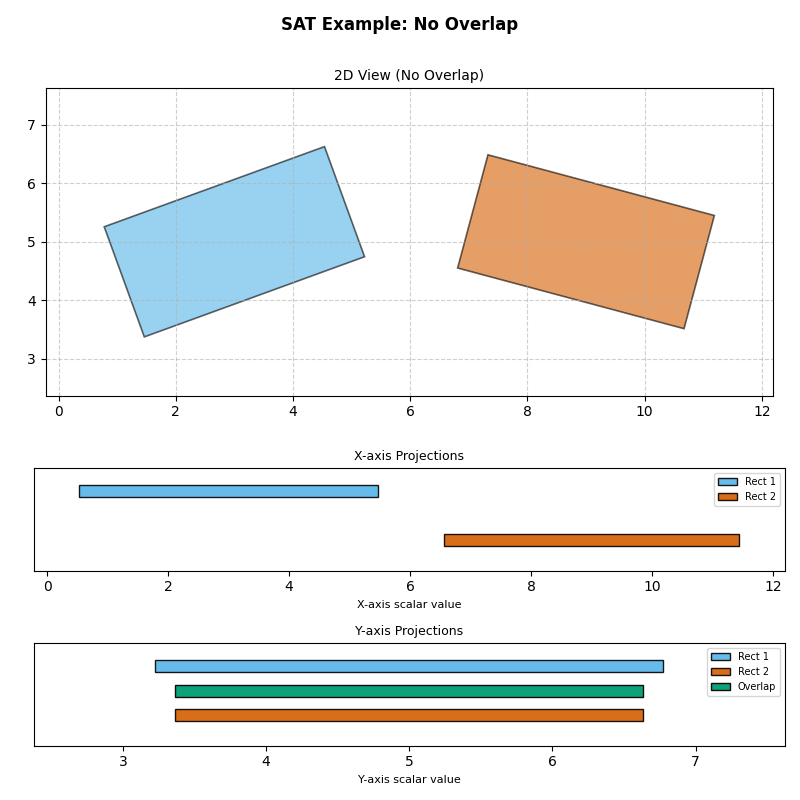
\includegraphics[width=\textwidth]{figures/sat_no_overlap_colored.png}
		\caption{Separation Axis Theorem with no overlap}
		\label{fig:1a_sat}
	\end{subfigure}
	\hfill
	\begin{subfigure}{0.45\textwidth}
		\centering
		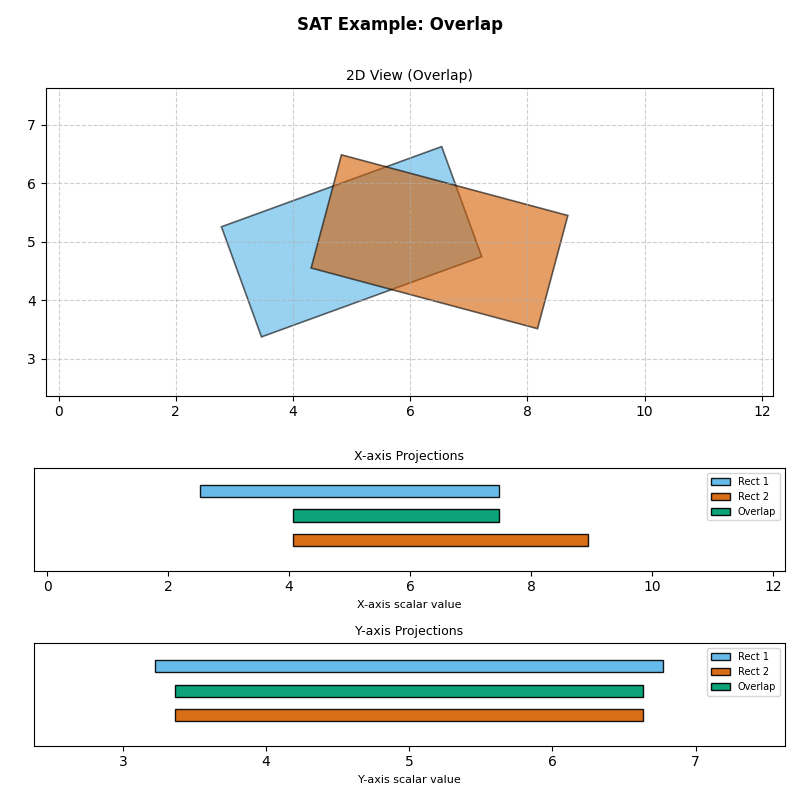
\includegraphics[width=\textwidth]{figures/sat_overlap_colored.png}
		\caption{Separation Axis Theorem with overlap}
		\label{fig:1b_sat}
	\end{subfigure}
	
	\caption{Separation Axis Theorem for oriented rectangles. Each figure consists of three subplots. The first subplot illustrates the spatial configuration of the rectangles. The second and third subplots show the projections of their principal axes onto the $x$- and $y$-axes, respectively. An overlap occurs when the projections intersect along both axes; the overlap is highlighted in black in the second and third subplots.}
	\label{fig:sat_theorem}
\end{figure}

During the search phase (lines~\ref{alg:start_pso_update}--\ref{alg:end_pso_update} of Algorithm~\ref{alg:pso_fixtures}), the velocity matrix $V_s$ and the position matrix $P_s$ associated with particle $s$ are iteratively updated according to the standard PSO update equations.

Whenever possible, constraint violations arising from updated fixture positions are mitigated through dedicated geometric repair procedures, as reported in lines~\ref{alg:start_fixing_geom}--\ref{alg:end_fixing_geom} of Algorithm~\ref{alg:pso_fixtures}. For each fixture, if its geometry lies partially or entirely outside the workpiece boundary, the nearest vertex of the workpiece polygon and the fixture vertex farthest from it are identified. The fixture is then translated by the minimum displacement required to satisfy the boundary constraint. The geometric repair strategy is limited to boundary violations, as these constraints are the most suitable for correction without adversely affecting the satisfaction of other constraints.

Lines~\ref{alg:start_fixing_type}--\ref{alg:end_fixing_type} of Algorithm~\ref{alg:pso_fixtures} report another constraints reparation strategy, where fixtures with type zero, representing unused fixtures, are directly assigned with the dummy lower-left corner coordinates $(\wtab,\htab)$, as in the CP model formulation (see Section~\ref{sec:second_cp_cons}), and are excluded from constraint violation evaluations.

To guide the search toward feasible positions, as illustrated in lines~\ref{alg:start_deb_eval}--\ref{alg:end_deb_eval} of Algorithm~\ref{alg:pso_fixtures}, candidate solutions are evaluated using Deb’s rules~\cite{deb2000efficient}:
\begin{itemize}
	\item Between two feasible solutions, retain the one with the higher objective value.
	\item Between a feasible and an infeasible solution, retain the feasible one.
	\item Between two infeasible solutions, retain the one with the lower constraint violation.
\end{itemize}

After updating the personal best position $P^*_s$ of each particle $s$ using Deb’s rules, the global best position $P^*$ of the swarm is updated accordingly. At the end of the final iteration, the best position found by the swarm is returned.


\section{Evaluation}
\label{sec:evaluation}
We evaluated the proposed resolution strategy on seven distinct workpieces: a stair step of a spiral staircase, a stair step of a simple staircase, a music speaker, a dashboard, a coffee table, a door, and a door with a porthole (see Table~\ref{tab:visual_results_first} and Table~\ref{tab:visual_results_second}).

The work center considered was equipped with 24 square fixtures with dimensions $145 \times 145$~mm and 12 rectangular fixtures with dimensions $180 \times 65$~mm. The minimum and maximum numbers of fixtures were set to $\nmin = 3$ and $\nmax = 6$, respectively, for all workpieces except the coffee table and the two door workpieces, which, due to their larger dimensions, required $\nmin = 6$ and $\nmax = 10$, and $\nmin = 10$ and $\nmax = 20$, respectively.

Both the CP and MIP models were implemented in MiniZinc version~2.9.5~\cite{nethercote2007minizinc}. The CP model was solved using the CP solvers Gecode~\cite{schulte2006gecode}, Chuffed~\cite{chuffed}, and OR-Tools~\cite{ortools}, whereas the MIP model was solved using the commercial solver Gurobi~\cite{gurobi}.

We also considered $\lns$, a variant of Gecode implementing Large Neighborhood Search (LNS)~\cite{pisinger2018large}, to solve the CP model, configuring it to explore the search space by randomly fixing 80\% of the decision variables corresponding to the $x$- and $y$-coordinates, adopting a constant restart strategy triggered every 1000 explored nodes.

All solvers were executed in single-threaded mode to ensure a fair comparison. The experiments were performed on a 64-bit Windows machine equipped with an Intel Core i5 processor and 16~GB of RAM.

Table~\ref{tab:objective_runtime} reports the values obtained for the objective function $\fdistarea$ for the different workpieces, together with the corresponding \emph{a posteriori} values of $\finer$, and the solve time $t_{solve}$ required to reach the optimal solution. 

Identical values of $\fdistarea$ do not necessarily correspond to identical values of $\finer$, as observed for the Dashboard workpiece. This is because the moments of inertia are highly sensitive to little displacement; therefore, if the solutions obtained by the solvers do not result in identical fixture placements, the value of $\finer$ may differ. 

Among the CP solvers, Gecode delivers the best overall performance, finding feasible solutions for all the considered workpieces, whereas Chuffed and OR-Tools fail to find feasible solutions for the two door workpieces.

$\lns$ achieves the best results for the two door workpieces, producing layouts that outperform those obtained by Gurobi with the MIP model. For the remaining workpieces, however, Gurobi finds solutions that are either superior or equivalent to those obtained by the CP solvers with respect to $\fdistarea$. This can be partly attributed to the use of continuous decision variables in the MIP model, which enlarges the feasible region and may therefore yield higher-quality solutions.

If we consider the information of the solve time presented in Table~\ref{tab:objective_runtime}, among the CP solvers, with an imposed time limit of 300~s, Chuffed is the most robust, finding the optimal solution in four of the seven instances, and it is the only CP solver able to prove optimality for the stiar step of the simple staircase. Gecode exhibits the greatest variability in performance, ranging from competitive runtimes on the easier instances to requiring 165.018~s for the speaker workpiece, while Chuffed and OR-Tools solve the same instance in only 0.106~s and 0.120~s, respectively.

Being a local-search-based approach, $\lns$ cannot prove optimality. Nevertheless, it reaches the same optimal value of $\fdistarea$ as the other CP solvers for the simpler workpieces and achieves the best value of $\finer$ in four out of the seven considered workpieces, demonstrating the effectiveness of a local search strategy.

\begin{landscape}
	
	\begin{table}[t]
		\centering
		\footnotesize
		\caption{Objective values for $\fdistarea$ and $\finer$, and solve time $t_{solve}$ in seconds to reach the best $\fdistarea$ solution. Timeout (300~s) is indicated by ``--''. Solutions where the solver reached optimality are marked with $^*$. For each workpiece, the maximum values of $\fdistarea$ and $\finer$ are highlighted in bold, including ties.}
		\label{tab:objective_runtime}
		\setlength{\tabcolsep}{2pt}
		\begin{tabular}{llccccc}
			\toprule
			Workpiece & Metric & Gecode & \lns & Chuffed & OR-Tools & Gurobi \\
			\midrule
			
			\multirow{3}{*}{\makecell{Stair step\\spiral staircase}} & $\fdistarea$ & $45655{}^*$ & $45655$ & $45655{}^*$ & $45655{}^*$ & $\mathbf{45662.155{}^*}$ \\
			& $\finer$ & \cellcolor{gray!15}$2.13968\times 10^{9}$ & \cellcolor{gray!15}$2.13968\times 10^{9}$ & \cellcolor{gray!15}$2.13960\times 10^{9}$ & \cellcolor{gray!15}$2.13968\times 10^{9}$ & \cellcolor{gray!15}$\mathbf{2.17089\times 10^{9}}$ \\
			& $t_{solve}$ & 0.559 & -- & 0.326 & 0.120 & 2.930 \\
			\midrule
			
			\multirow{3}{*}{\makecell{Stair step\\simple staircase}} & $\fdistarea$ & $72823$ & $72823$ & $72823{}^*$ & $72721$ & $\mathbf{72826.000{}^*}$ \\
			& $\finer$ & \cellcolor{gray!15}$6.76573\times 10^{9}$ & \cellcolor{gray!15}$6.76573\times 10^{9}$ & \cellcolor{gray!15}$6.76530\times 10^{9}$ & \cellcolor{gray!15}$6.48172\times 10^{9}$ & \cellcolor{gray!15}$\mathbf{6.76638\times 10^{9}}$ \\
			& $t_{solve}$ & -- & -- & 3.386 & -- & 0.220 \\
			\midrule
			
			\multirow{3}{*}{\makecell{Dashboard}} & $\fdistarea$ & $\mathbf{55582{}^*}$ & $\mathbf{55582}$ & $\mathbf{55582{}^*}$ & $\mathbf{55582{}^*}$ & $\mathbf{55582.000{}^*}$ \\
			& $\finer$ & \cellcolor{gray!15}$\mathbf{7.10094\times 10^{9}}$ & \cellcolor{gray!15}$\mathbf{7.10094\times 10^{9}}$ & \cellcolor{gray!15}$7.08735\times 10^{9}$ & \cellcolor{gray!15}$7.08735\times 10^{9}$ & \cellcolor{gray!15}$7.08735\times 10^{9}$ \\
			& $t_{solve}$ & 0.044 & -- & 0.057 & 0.102 & 0.157 \\
			\midrule
			
			\multirow{3}{*}{\makecell{Speaker}} & $\fdistarea$ & $\mathbf{49548{}^*}$ & $\mathbf{49548}$ & $\mathbf{49548{}^*}$ & $\mathbf{49548{}^*}$ & $\mathbf{49548.000{}^*}$ \\
			& $\finer$ & \cellcolor{gray!15}$\mathbf{2.93433\times 10^{9}}$ & \cellcolor{gray!15}$\mathbf{2.93433\times 10^{9}}$ & \cellcolor{gray!15}$\mathbf{2.93433\times 10^{9}}$ & \cellcolor{gray!15}$\mathbf{2.93433\times 10^{9}}$ & \cellcolor{gray!15}$\mathbf{2.93433\times 10^{9}}$ \\
			& $t_{solve}$ & 165.018 & -- & 0.106 & 0.120 & 0.126 \\
			\midrule
			
			\multirow{3}{*}{\makecell{Coffee table}} & $\fdistarea$ & $137262$ & $185351$ & $192711$ & $122920$ & $\mathbf{201686.505}$ \\
			& $\finer$ & \cellcolor{gray!15}$2.20750\times 10^{10}$ & \cellcolor{gray!15}$2.19967\times 10^{10}$ & \cellcolor{gray!15}$\mathbf{2.21449\times 10^{10}}$ & \cellcolor{gray!15}$9.10490\times 10^{9}$ & \cellcolor{gray!15}$2.19472\times 10^{10}$ \\
			& $t_{solve}$ & -- & -- & -- & -- & -- \\
			\midrule
			
			\multirow{3}{*}{\makecell{Door}} & $\fdistarea$ & $261757$ & $\mathbf{521632}$ & -- & -- & $355744.000$ \\
			& $\finer$ & \cellcolor{gray!15}$1.08442\times 10^{11}$ & \cellcolor{gray!15}$\mathbf{1.52925\times 10^{11}}$ & \cellcolor{gray!15}-- & \cellcolor{gray!15}-- & \cellcolor{gray!15}$1.17690\times 10^{11}$ \\
			& $t_{solve}$ & -- & -- & -- & -- & -- \\
			\midrule
			
			\multirow{3}{*}{\makecell{Door\\with porthole}} & $\fdistarea$ & $261759$ & $\mathbf{393343}$ & -- & -- & $298186.000$ \\
			& $\finer$ & \cellcolor{gray!15}$1.08422\times 10^{11}$ & \cellcolor{gray!15}$\mathbf{1.52861\times 10^{11}}$ & \cellcolor{gray!15}-- & \cellcolor{gray!15}-- & \cellcolor{gray!15}$1.39714\times 10^{11}$ \\
			& $t_{solve}$ & -- & -- & -- & -- & -- \\
			
			\bottomrule
		\end{tabular}
	\end{table}
	
\end{landscape}

The Q-learning based algorithm was implemented in Python~3.11.9 using the Gymnasium library version~1.3.0. The agent was trained on all the considered workpieces for 200 episodes, each consisting of 20 steps, using the following hyperparameters: learning rate $\alpha = 0.1$, discount factor $\gamma = 0.99$, initial exploration rate $\epsilon = 1.0$, and exploration decay factor $\rho = 0.995$.

Table~\ref{tab:comparison} reports the results obtained for the different workpieces, comparing the corresponding values of the moment of inertia with those achieved by the best CP solver and the MIP model.

Overall, the Q-learning based algorithm does not outperform either the CP or the MIP model. On average, the values of $\finer$ obtained by Q-learning are 13\% lower than those achieved by CP and 8\% lower than those obtained with MIP. The only exception is the door with a porthole workpiece, for which Q-learning outperforms the solution returned by Gurobi for the MIP model.


\begin{table}[t]
	\centering
	\footnotesize
	\caption{Objective values $\finer$ comparison: CP solvers (best among Gecode, LNS, Chuffed, OR-Tools), MIP solver (Gurobi), and RL approach. For each workpiece, the maximum value is highlighted in bold.}
	\label{tab:comparison}
	\setlength{\tabcolsep}{5pt}
	\begin{tabular}{cccc}
		\toprule
		Workpiece & CP model & MIP model & Q-learning \\
		\midrule
		
		\makecell{Stair step\\spiral staircase} & $2.13968\times 10^{9}$ & $\mathbf{2.17089\times 10^{9}}$ & $1.93822\times 10^{9}$ \\
		\midrule
		
		\makecell{Stair step\\simple staircase} & $6.76573\times 10^{9}$ & $\mathbf{6.76638\times 10^{9}}$ & $5.65433\times 10^{9}$ \\
		\midrule
		
		\makecell{Dashboard} & $\mathbf{7.10094\times 10^{9}}$ & $7.08735\times 10^{9}$ & $6.65446\times 10^{9}$ \\
		\midrule
		
		\makecell{Speaker} & $\mathbf{2.93433\times 10^{9}}$ & $\mathbf{2.93433\times 10^{9}}$ & $2.81248\times 10^{9}$ \\
		\midrule
		
		\makecell{Coffee table} & $\mathbf{2.29750\times 10^{10}}$ & $2.19472\times 10^{10}$ & $1.56444\times 10^{10}$ \\
		\midrule
		
		\makecell{Door} & $\mathbf{1.52925\times 10^{11}}$ & $1.17690\times 10^{11}$ & $1.14387\times 10^{11}$ \\
		\midrule
		
		\makecell{Door\\with porthole} & $\mathbf{1.52861\times 10^{11}}$ & $1.39714\times 10^{11}$ & $1.45467\times 10^{11}$ \\
		
		\bottomrule
	\end{tabular}
\end{table}


\begin{figure}[t]
	\centering
	\begin{subfigure}[b]{\textwidth}
		\centering
		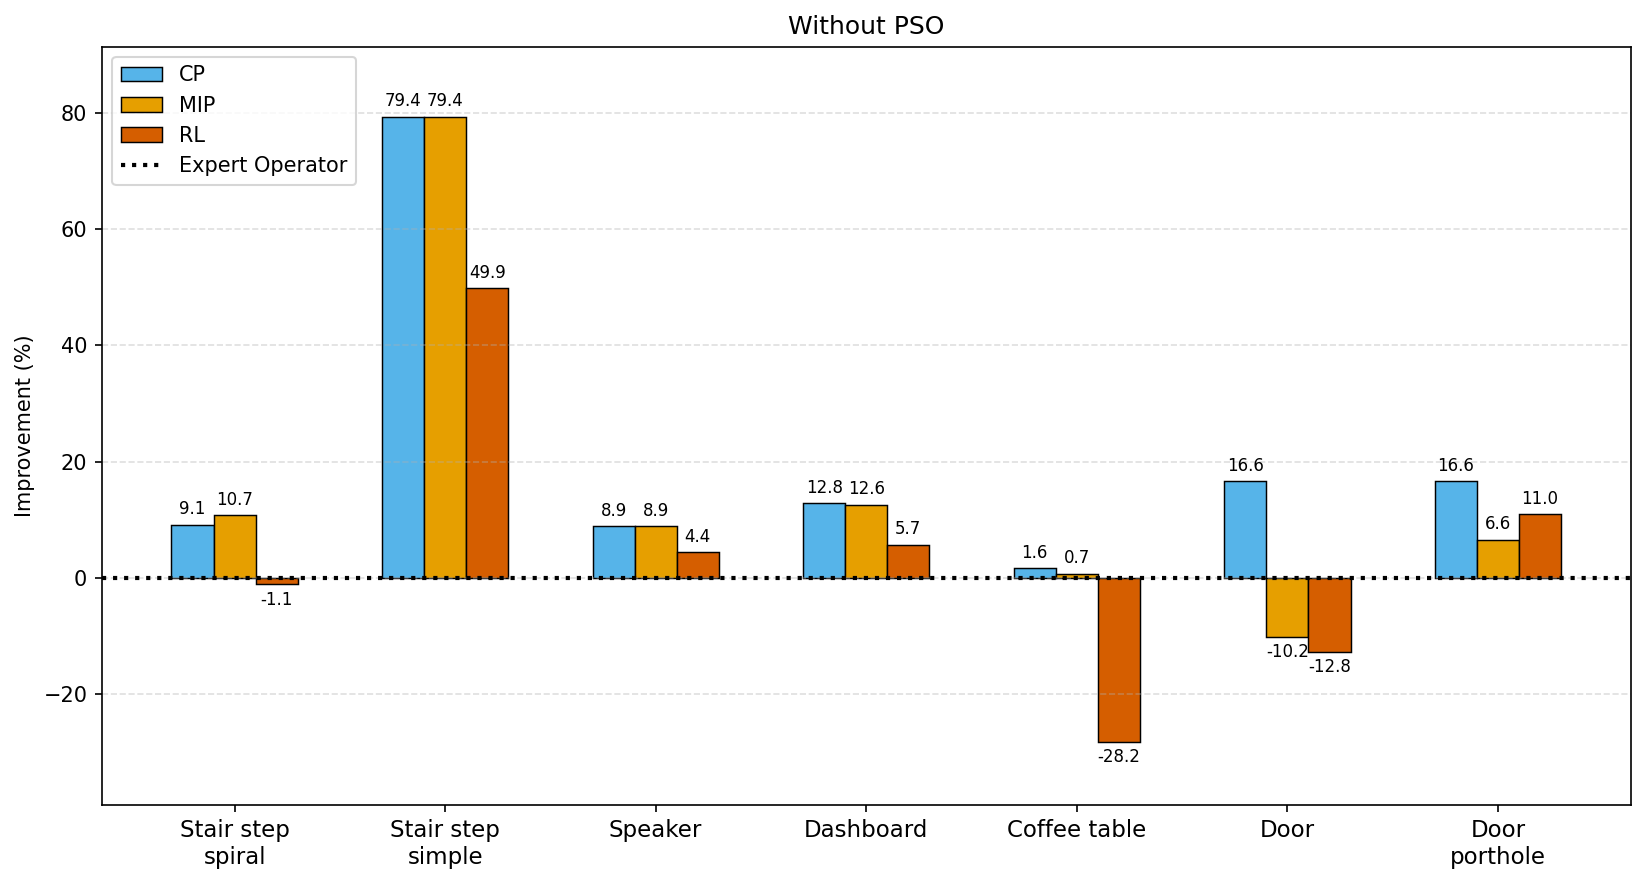
\includegraphics[width=\textwidth]{figures/comparison_plot_1.png}
		\caption{Percentage improvement over expert operator}
		\label{fig:comparison_plot1}
	\end{subfigure}
	%\hspace{1.5cm}
	\begin{subfigure}[b]{\textwidth}
		\centering
		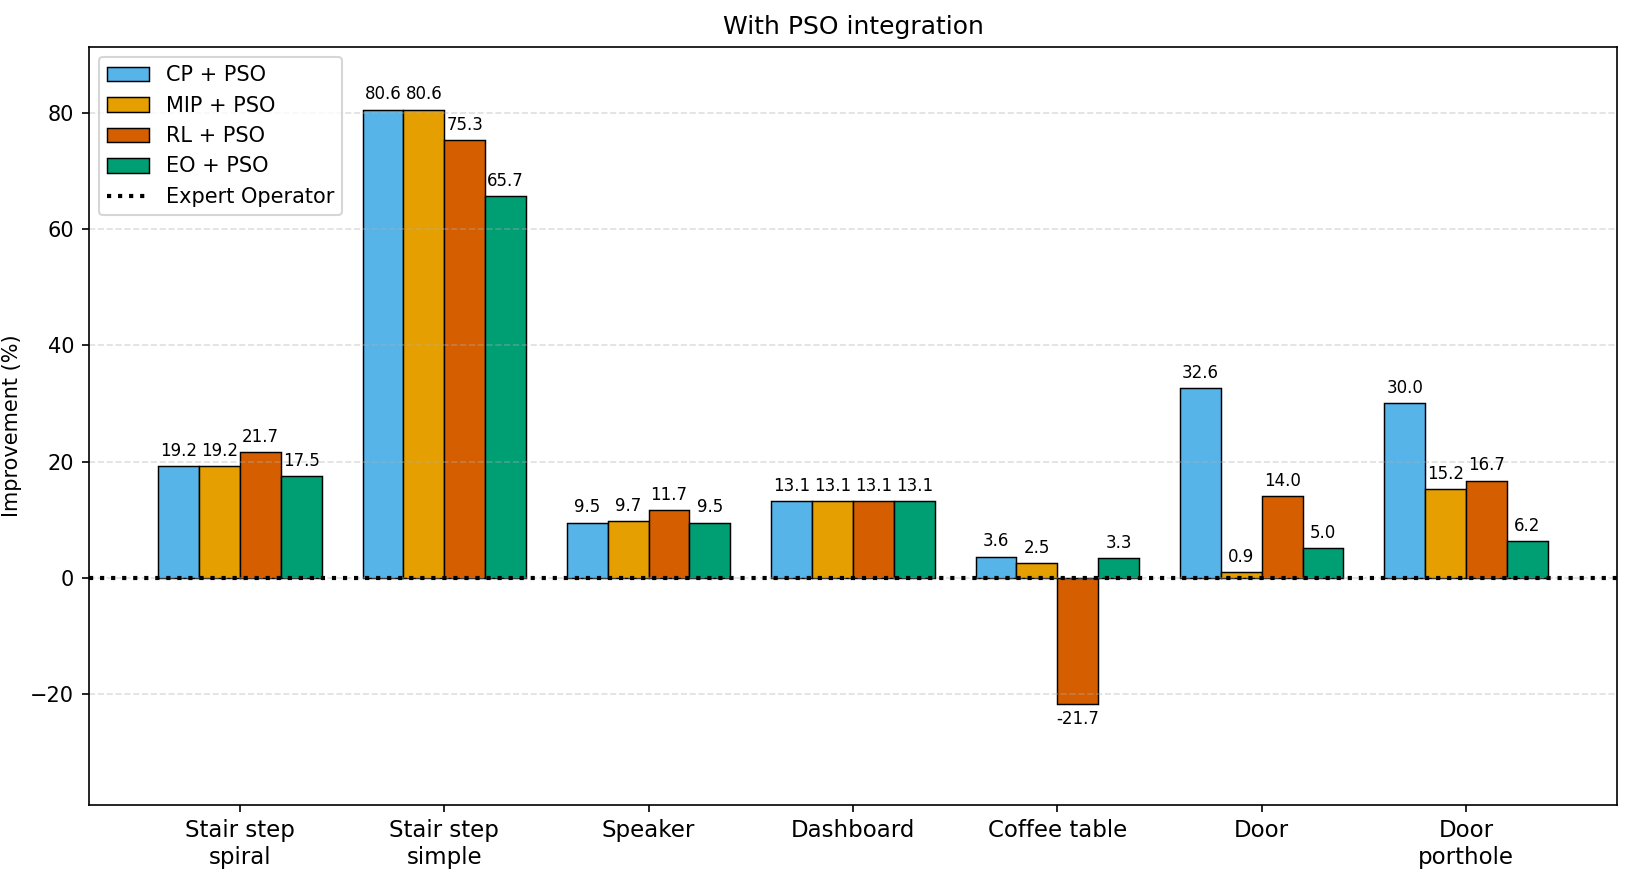
\includegraphics[width=\textwidth]{figures/comparison_plot_2.png}
		\caption{Percentage improvement over expert operator after PSO refinement}
		\label{fig:comparison_plot2}
	\end{subfigure}
	\caption{Percentage improvement relative to the solution provided by the expert operator. The first plot illustrates the improvements achieved by the CP model, MIP model and Q-learning algorithm without PSO integration, whereas the second plot presents the improvements obtained with PSO integration, alongside the improvement of the expert operator's solution when combined with PSO.}
	\label{fig:improvement}
\end{figure}

For each workpiece, the best CP and MIP solutions in terms of $\finer$, together with the Q-learning solution, were used as initial ones for the PSO algorithm. 

To enable direct integration into the target industrial system, the PSO algorithm was implemented in Java~18.0.2. Its hyper-parameters were tuned using the Optuna framework~\cite{akiba2019optuna}, yielding the following configuration: $\swarmsize = 1374$, $\maxiter = 2912$, $w = 0.669$, $c_1 = 2.385$, and $c_2 = 0.558$.

Figure~\ref{fig:improvement} shows the percentage improvement in $\finer$ with respect to the layout proposed by an expert operator. The first plot (Figure~\ref{fig:comparison_plot1}) reports the improvements achieved by the CP model, the MIP model, and the Q-learning algorithm before PSO refinement, whereas the second plot (Figure~\ref{fig:comparison_plot2}) shows the corresponding results after PSO refinement, including those obtained by initializing PSO from the expert layout.

The largest workpieces, namely the coffee table, the door, and the door with porthole, represent the most challenging instances. Among the considered approaches, the CP model consistently achieves the best improvements over the expert layout and is the only one that improves upon the expert solution for the door workpiece.

The Q-learning algorithm outperforms the expert layout in four of the seven considered workpieces. The integration with PSO further improves the solutions generated by the Q-learning algorithm for the stair step of the spiral staircase and the door, allowing them to surpass the expert layout. Conversely, when initialized with the Q-learning solution for the Coffee table, which represents the weakest initial layout, PSO achieves only marginal improvements, highlighting the importance of providing a high-quality starting solution.

The plot in Figure~\ref{fig:comparison_plot2} reports in green the improvement achieved by initializing PSO with the expert operator layout, and for all the considered workpieces, PSO generates layouts that outperform the expert solution, demonstrating its effectiveness as a refinement technique.

\begin{landscape}
	\begin{table}[t]
		\centering
		\renewcommand{\arraystretch}{1.3}
		\setlength{\tabcolsep}{3pt}
		\caption{Summary of the best solutions, corresponding solution providers, and moment of inertia values for the first four workpieces. 
			The workpiece perimeter is shown with solid lines. Dashed lines indicate areas to be extruded, fixture regions are marked with diagonal hatching, and supporting bars are shown as shaded rectangles.}
		\label{tab:visual_results_first}
		\begin{tabular}{c c c c c}
			\hline
			\textbf{Workpiece} & \textbf{Expert Operator} & \textbf{Best CP/MIP} & \textbf{Q-learning} & \textbf{Best with PSO} \\
			\hline
			
			\makecell{Spiral stair step} & 
			\makecell{$1.96057\times 10^{9}$ \\ 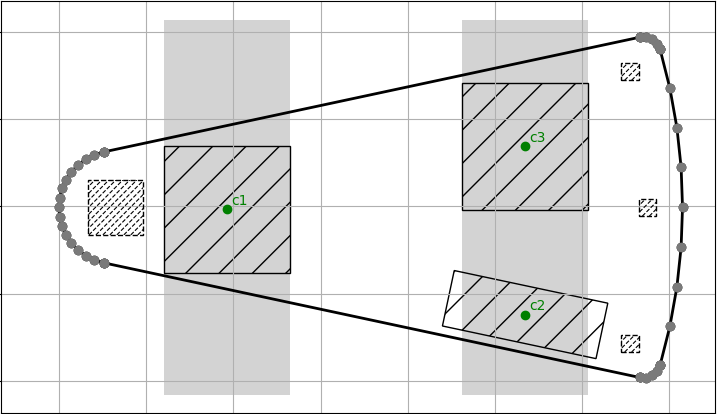
\includegraphics[width=0.18\linewidth]{figures/spiral_stair_step_expert_operator.png}} & 
			\makecell{MIP: $2.17089\times 10^{9}$ \\ 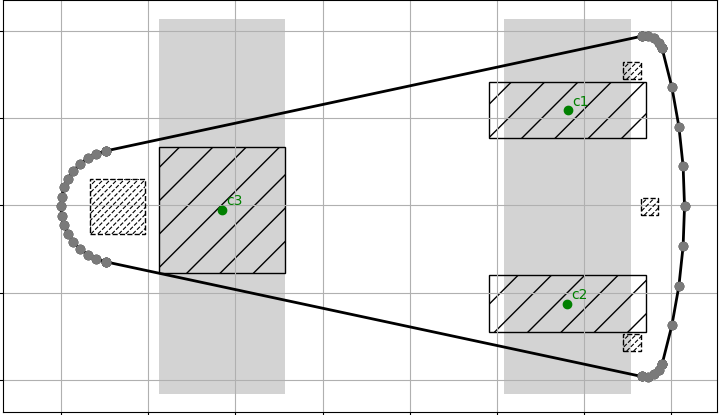
\includegraphics[width=0.18\linewidth]{figures/spiral_stair_step_mip_model_gurobi.png}} & 
			\makecell{$1.93822\times 10^{9}$ \\ 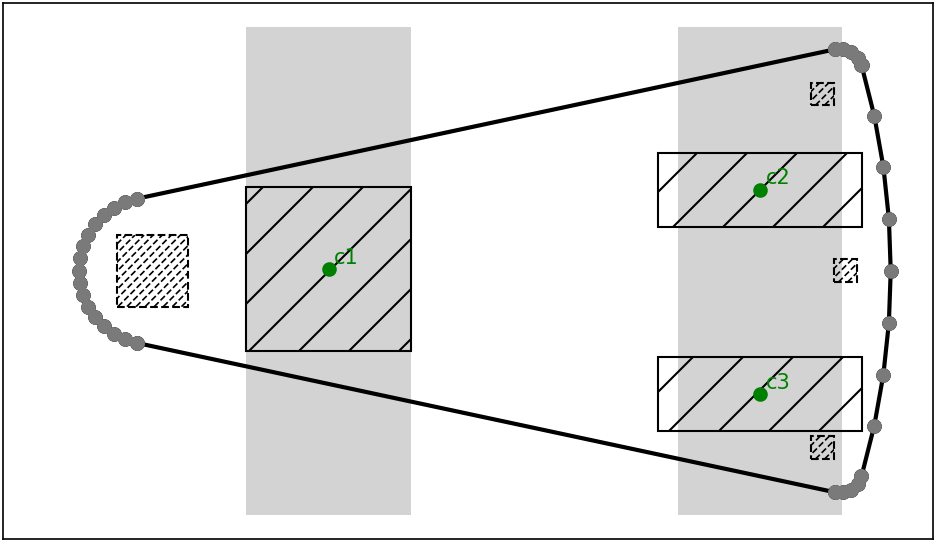
\includegraphics[width=0.18\linewidth]{figures/spiral_stair_step_rl.png}} & 
			\makecell{RL: $2.38520\times 10^{9}$ \\ 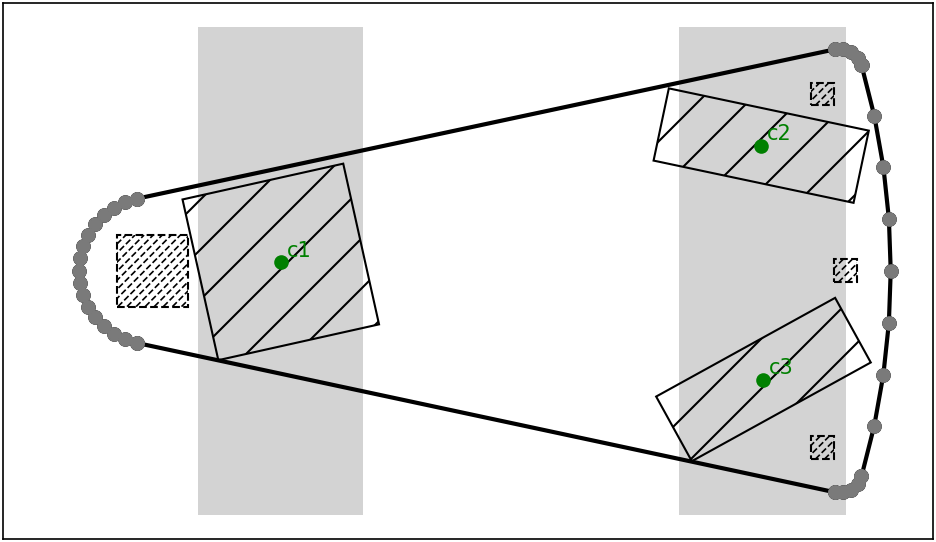
\includegraphics[width=0.18\linewidth]{figures/spiral_stair_step_pso_rl_pso.png}} \\
			\hline
			
			\makecell{Simple stair step} & 
			\makecell{$3.77213\times 10^{9}$ \\ 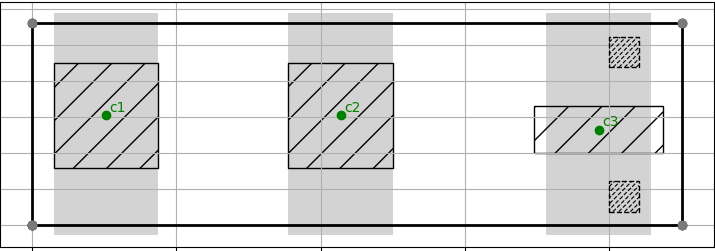
\includegraphics[width=0.18\linewidth]{figures/simple_stair_step_expert_operator.png}} & 
			\makecell{MIP: $6.76638\times 10^{9}$ \\ 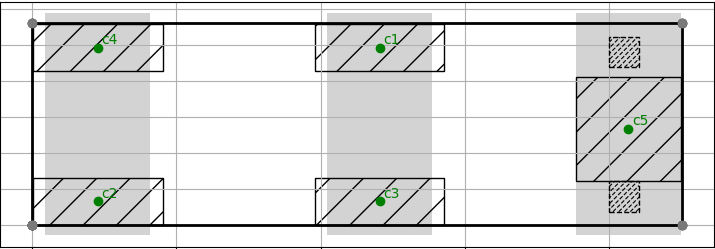
\includegraphics[width=0.18\linewidth]{figures/simple_stair_step_mip_model_gurobi.png}} & 
			\makecell{$5.65433\times 10^{9}$ \\ 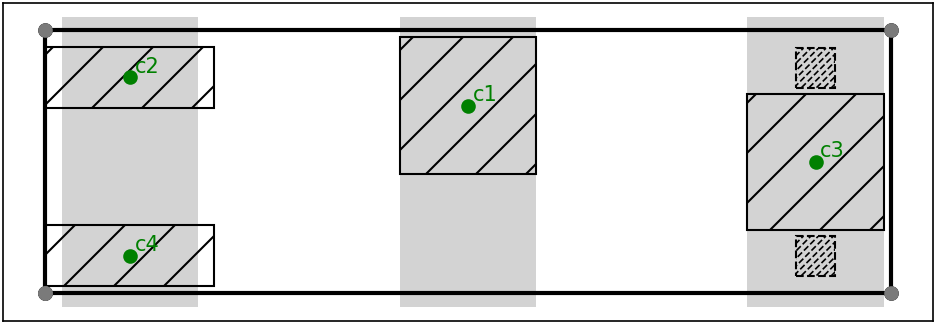
\includegraphics[width=0.18\linewidth]{figures/simple_stair_step_rl.png}} & 
			\makecell{CP: $6.81108\times 10^{9}$ \\ 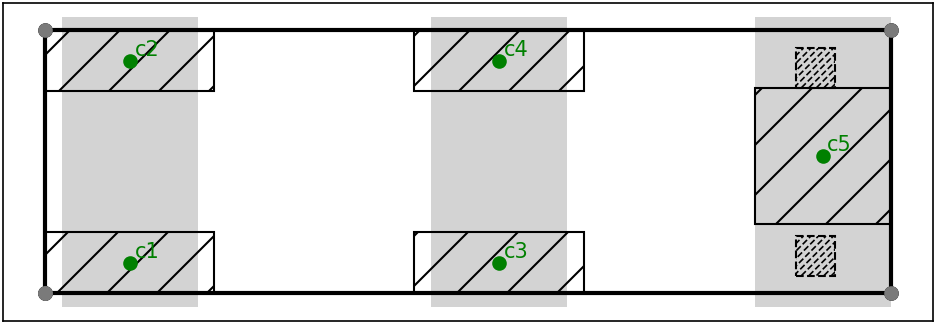
\includegraphics[width=0.18\linewidth]{figures/simple_stair_step_pso_cp_pso.png}} \\
			\hline
			
			\makecell{Dashboard} & 
			\makecell{$6.29544\times 10^{9}$ \\ 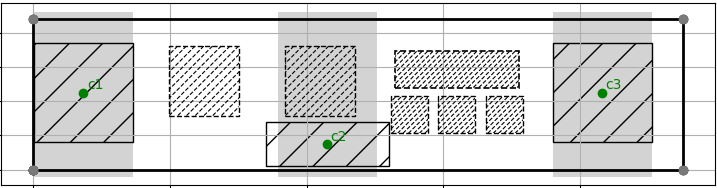
\includegraphics[width=0.18\linewidth]{figures/dashboard_expert_operator.png}} & 
			\makecell{CP: $7.10094\times 10^{9}$ \\ 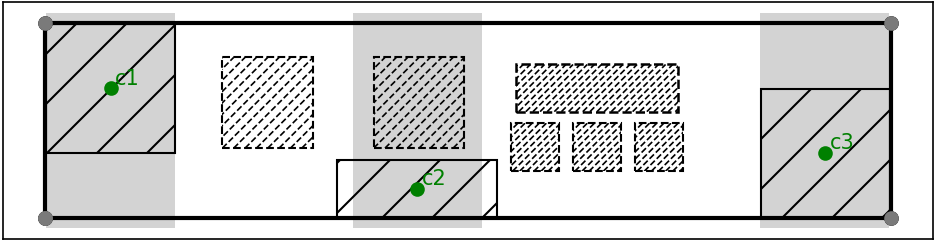
\includegraphics[width=0.18\linewidth]{figures/dashboard_cp_model_gecode.png}} & 
			\makecell{$6.65446\times 10^{9}$ \\ 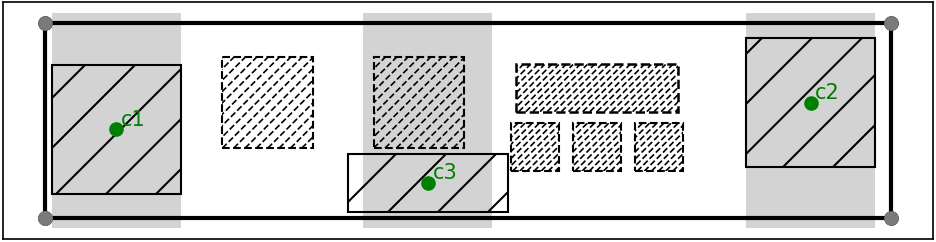
\includegraphics[width=0.18\linewidth]{figures/dashboard_rl.png}} & 
			\makecell{CP: $7.12226\times 10^{9}$ \\ 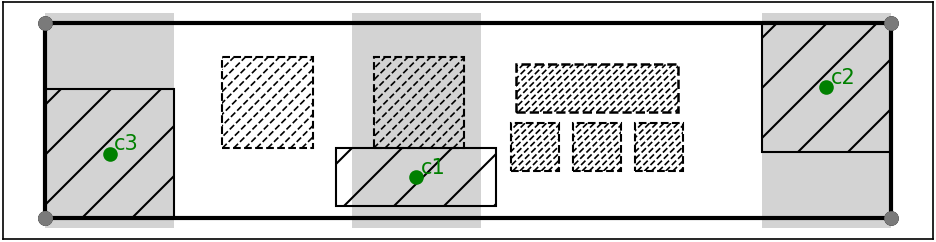
\includegraphics[width=0.18\linewidth]{figures/dashboard_pso_cp_pso.png}} \\
			\hline
			
			\makecell{Speaker} & 
			\makecell{$2.69490\times 10^{9}$ \\ 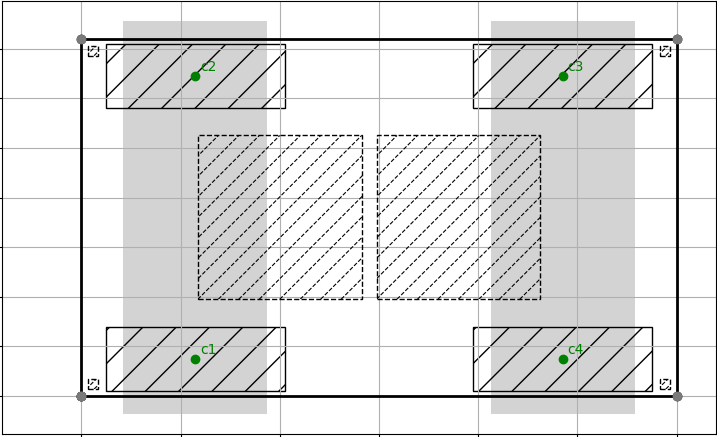
\includegraphics[width=0.18\linewidth]{figures/speaker_expert_operator.png}} & 
			\makecell{CP, MIP: $2.93433\times 10^{9}$ \\ 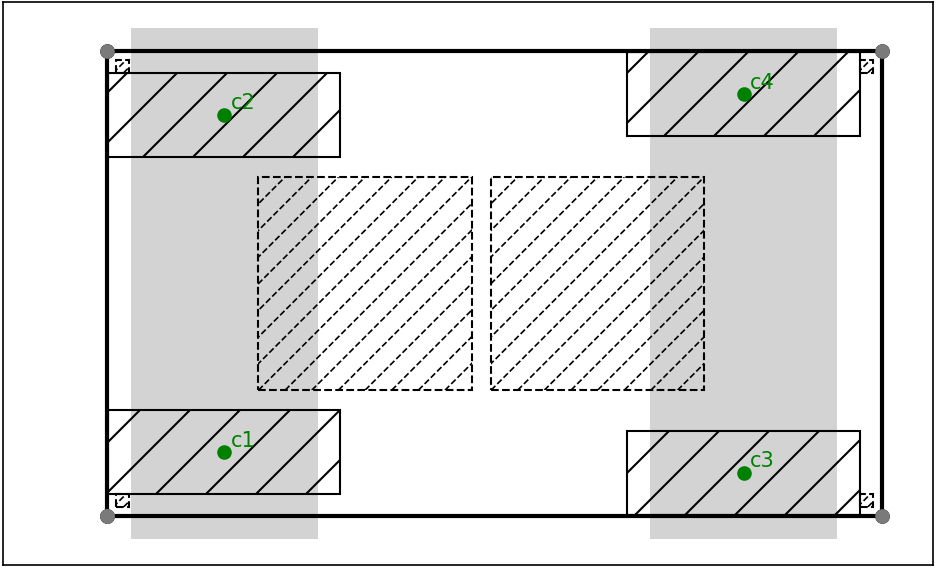
\includegraphics[width=0.18\linewidth]{figures/speaker_cp_model_gecode.png}} & 
			\makecell{$2.81248\times 10^{9}$ \\ 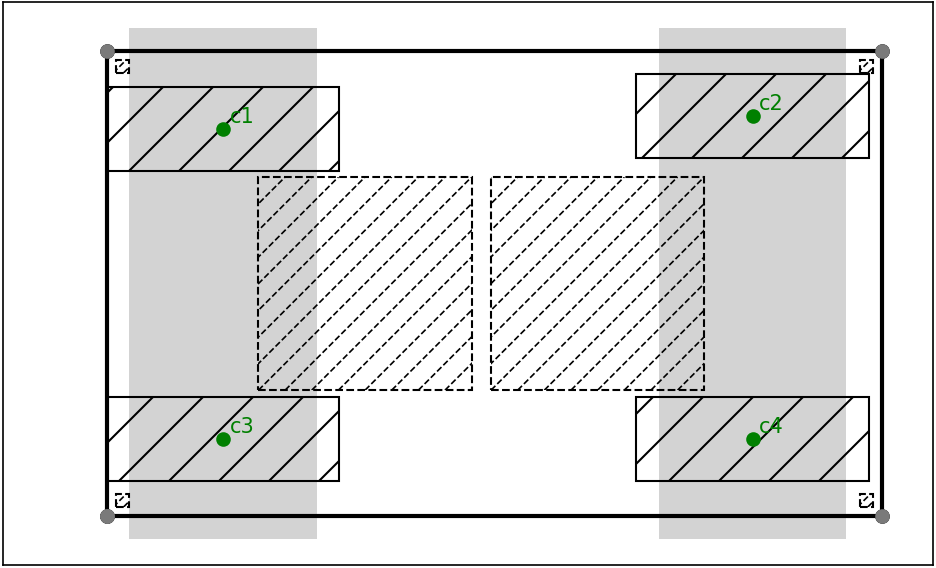
\includegraphics[width=0.18\linewidth]{figures/speaker_rl.png}} & 
			\makecell{RL: $3.00979\times 10^{9}$ \\ 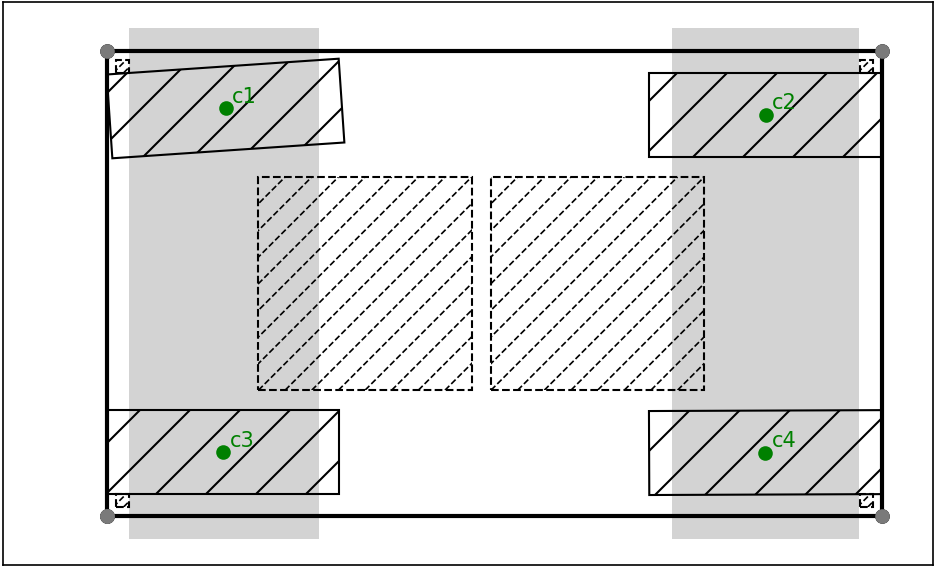
\includegraphics[width=0.18\linewidth]{figures/speaker_pso_rl_pso.png}} \\
			\hline
			
		\end{tabular}
	\end{table}
	
	\begin{table}[t]
		\centering
		\renewcommand{\arraystretch}{1.3}
		\setlength{\tabcolsep}{3pt}
		\caption{Summary of the best solutions, corresponding solution providers, and moment of inertia values for the remaining three workpieces. 
			The workpiece perimeter is shown with solid lines. Dashed lines indicate areas to be extruded, fixture regions are marked with diagonal hatching, and supporting bars are shown as shaded rectangles.}
		\label{tab:visual_results_second}
		\begin{tabular}{c c c c c}
			\hline
			\textbf{Workpiece} & \textbf{Expert Operator} & \textbf{Best CP/MIP} & \textbf{Q-learning} & \textbf{Best with PSO} \\
			\hline
			
			\makecell{Coffee table} & 
			\makecell{$2.17954\times 10^{10}$ \\ 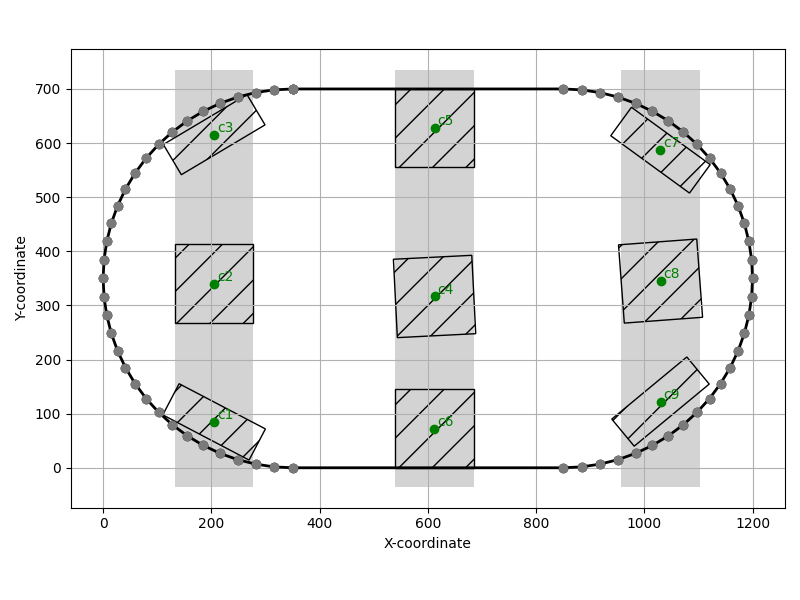
\includegraphics[width=0.18\linewidth]{figures/coffee_table_expert_operator.png}} & 
			\makecell{CP: $2.21449\times 10^{10}$ \\ 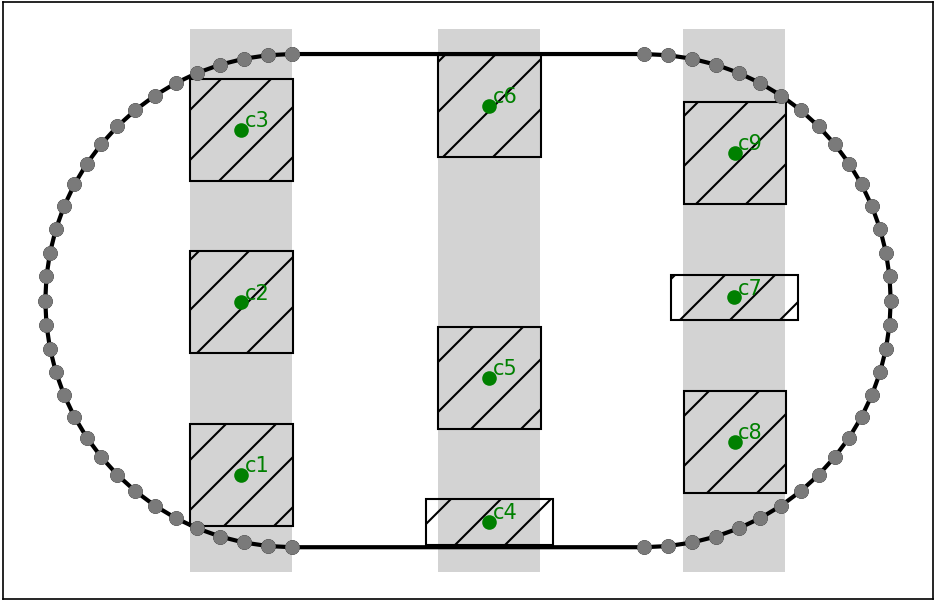
\includegraphics[width=0.18\linewidth]{figures/coffee_table_cp_model_chuffed.png}} & 
			\makecell{$1.56444\times 10^{10}$ \\ 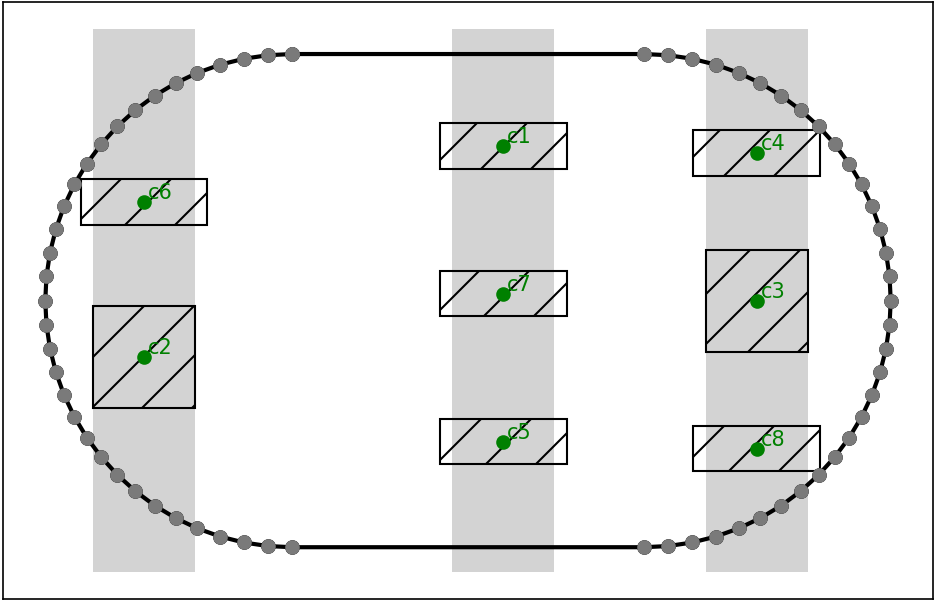
\includegraphics[width=0.18\linewidth]{figures/coffee_table_rl.png}} & 
			\makecell{CP: $2.25868\times 10^{10}$ \\ 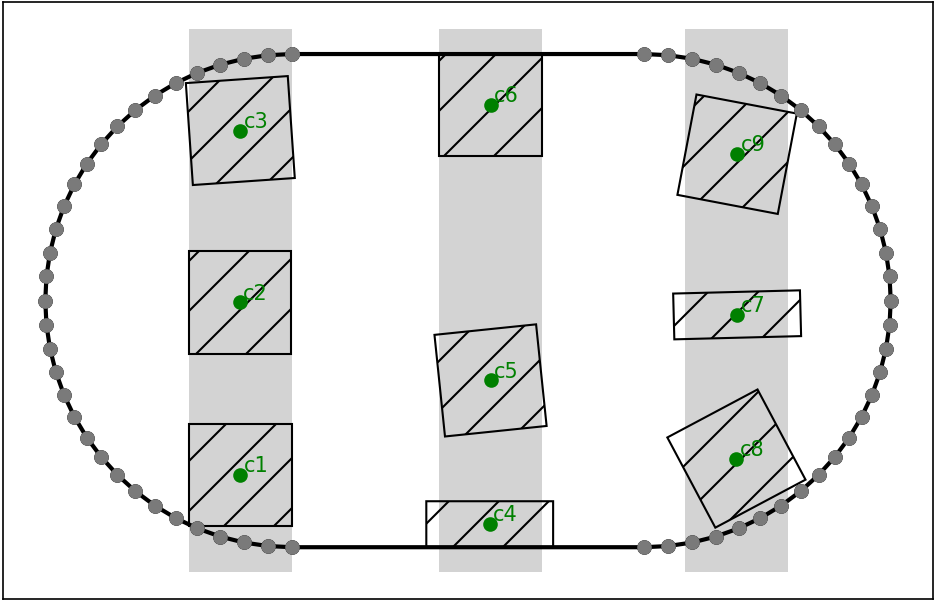
\includegraphics[width=0.18\linewidth]{figures/coffee_table_pso_cp_pso.png}} \\
			\hline
			
			\makecell{Door} & 
			\makecell{$1.31109\times 10^{11}$ \\ 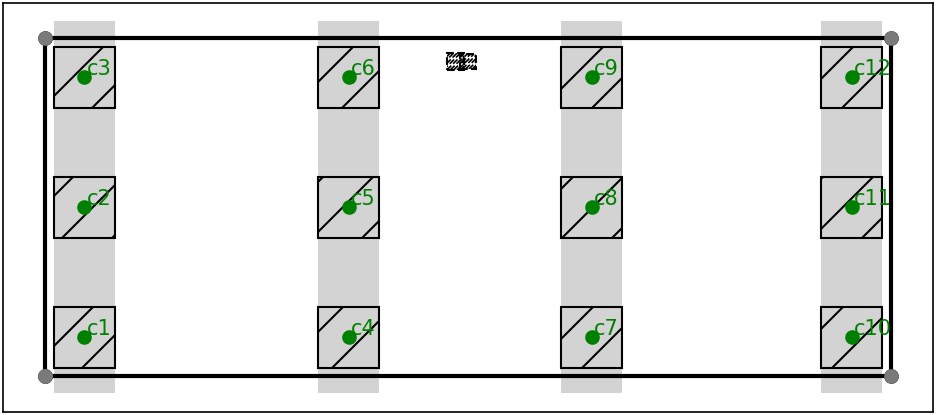
\includegraphics[width=0.18\linewidth]{figures/door_expert_operator.png}} & 
			\makecell{CP: $1.52925\times 10^{11}$ \\ 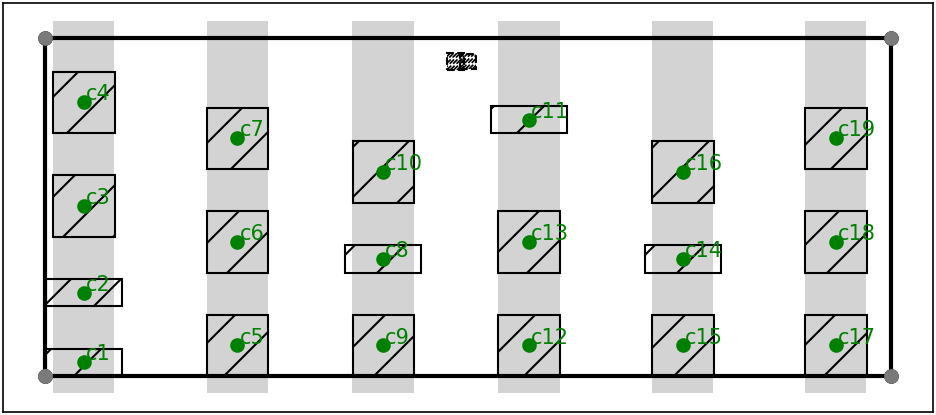
\includegraphics[width=0.18\linewidth]{figures/door_LNS_cp_model_gecode.png}} & 
			\makecell{$1.14387\times 10^{11}$ \\ 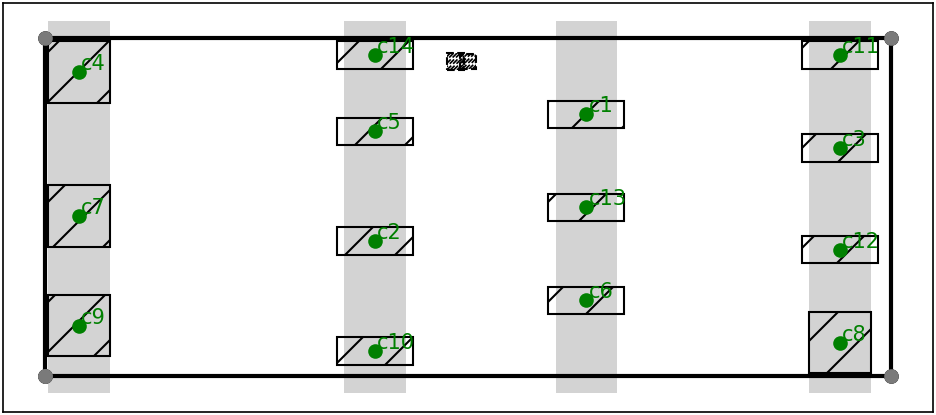
\includegraphics[width=0.18\linewidth]{figures/door_rl.png}} & 
			\makecell{CP: $1.73826\times 10^{11}$ \\ 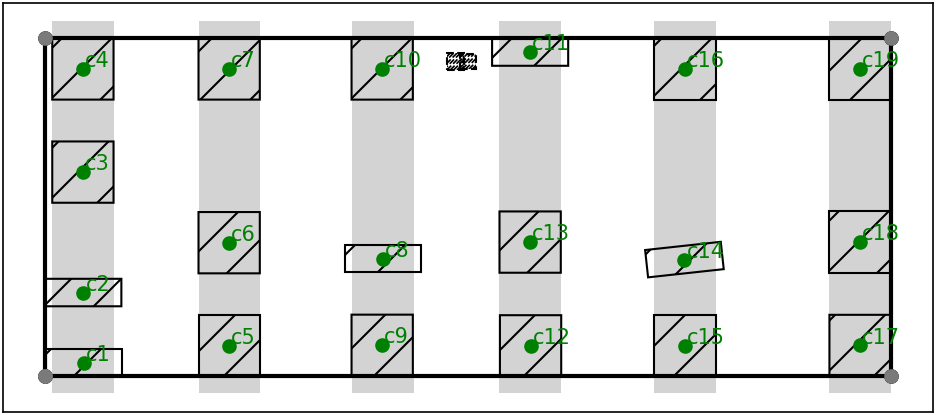
\includegraphics[width=0.18\linewidth]{figures/door_pso_cp_pso.png}} \\
			\hline
			
			\makecell{Door porthole} & 
			\makecell{$1.31109\times 10^{11}$ \\ 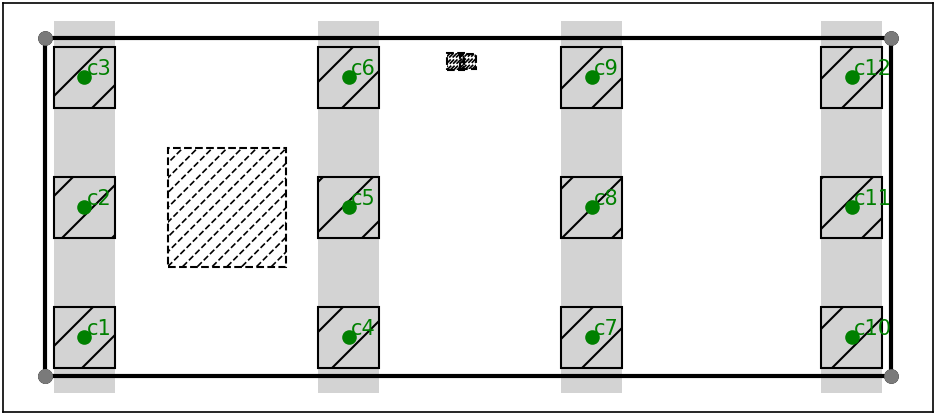
\includegraphics[width=0.18\linewidth]{figures/door_porthole_expert_operator.png}} & 
			\makecell{CP: $1.52861\times 10^{11}$ \\ 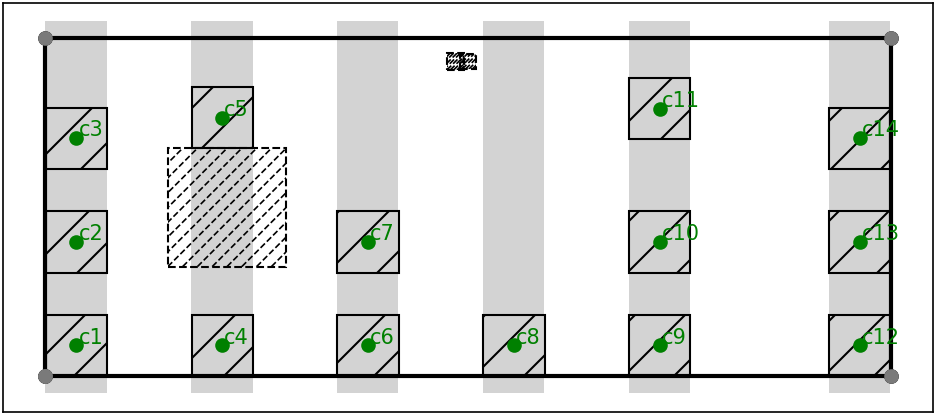
\includegraphics[width=0.18\linewidth]{figures/door_porthole_LNS_cp_model_gecode.png}} & 
			\makecell{$1.45467\times 10^{11}$ \\ 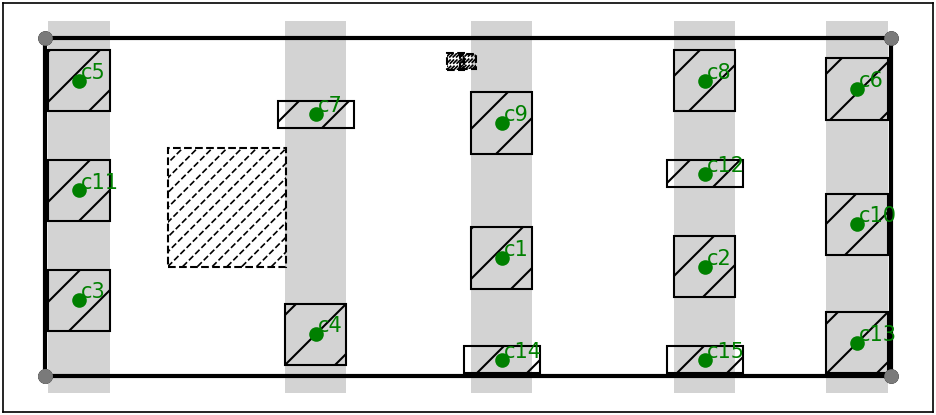
\includegraphics[width=0.18\linewidth]{figures/door_porthole_rl.png}} & 
			\makecell{CP: $1.70507\times 10^{11}$ \\ 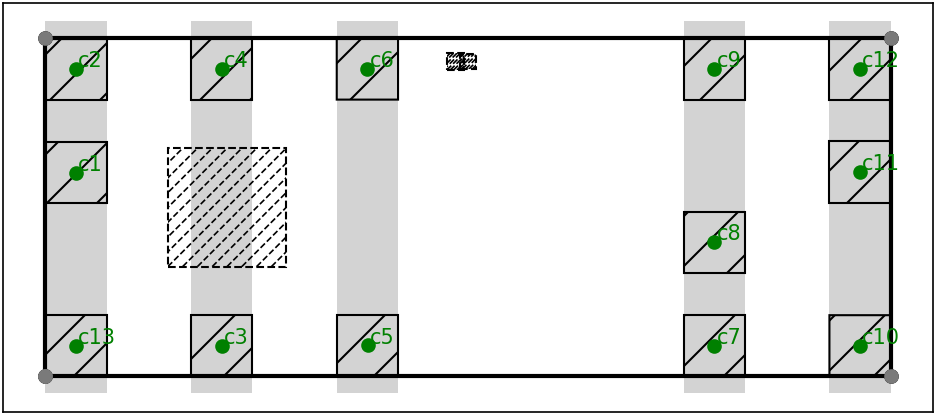
\includegraphics[width=0.18\linewidth]{figures/door_porthole_pso_cp_pso.png}} \\
			\hline
			
		\end{tabular}
	\end{table}
\end{landscape}

Tables~\ref{tab:visual_results_first} and ~\ref{tab:visual_results_second} report visual comparisons of the best solutions obtained with the CP model, the MIP model, and the Q-learning algorithm for the different workpieces, together with the corresponding solutions refined by PSO. Note that, in the figures, the support bars can be positioned beneath the areas to be extruded, since the fixture height prevents collisions between the cutting tools and the bars.

The layouts proposed by the Q-learning algorithm are qualitatively similar to those obtained with the CP and MIP models. An exception is the coffee table, where Q-learning tends to favour the placement of a larger number of rectangular fixtures instead of square ones, resulting in a lower value for the moment of inertia.

Rotation plays an important role in the stair step of the spiral staircase and coffee table workpieces, where fixture orientation improves adherence to the workpiece boundary. For the Speaker workpiece, the PSO refinement of the Q-learning solution introduces only a slight rotation of the upper-left fixture, yielding the marginal improvement reported in Figure~\ref{fig:improvement}.

The stair step of the simple staircase exhibits the largest improvement over the expert layout. This is mainly due to the use of a larger number of fixtures, five for the CP and MIP models and four for the Q-learning algorithm, compared with the three fixtures used by the expert operator.

For both the door and the door with a porthole workpieces, the expert operator adopts a symmetric fixture layout, whereas the PSO refinement tends to move the fixtures farther from the workpiece centre. Since the principal moments of inertia are maximised when the fixtures are placed away from the symmetry axes, this configuration yields higher values of $\finer$. Moreover, in the door workpiece, the expert layout relies exclusively on square fixtures, whereas the optimization strategies increase the number of fixtures using even rectangular ones, thereby increasing the supported area of the workpiece.

Overall, the best trade-off between computational time and solution quality is achieved by integrating the CP model with PSO. The CP formulation is expected to scale better to problems involving additional fixture types and multiple areas to be extruded owing to the stronger propagation of the \texttt{diffn} global constraint and the fact that type and overlap decisions are modeled through discrete variables that cannot be relaxed, unlike the $x$ and $y$ variables in the MIP formulation.


